%%% The main file. It contains definitions of basic parameters and includes all other parts.

%% Settings for single-side (simplex) printing
% Margins: left 40mm, right 25mm, top and bottom 25mm
% (but beware, LaTeX adds 1in implicitly)
\documentclass[12pt,a4paper]{report}
\setlength\textwidth{145mm}
\setlength\textheight{247mm}
\setlength\oddsidemargin{15mm}
\setlength\evensidemargin{15mm}
\setlength\topmargin{0mm}
\setlength\headsep{0mm}
\setlength\headheight{0mm}
% \openright makes the following text appear on a right-hand page
\let\openright=\clearpage

%% Settings for two-sided (duplex) printing
% \documentclass[12pt,a4paper,twoside,openright]{report}
% \setlength\textwidth{145mm}
% \setlength\textheight{247mm}
% \setlength\oddsidemargin{14.2mm}
% \setlength\evensidemargin{0mm}
% \setlength\topmargin{0mm}
% \setlength\headsep{0mm}
% \setlength\headheight{0mm}
% \let\openright=\cleardoublepage

%% Generate PDF/A-2u
\usepackage[a-2u]{pdfx}

%% Character encoding: usually latin2, cp1250 or utf8:
\usepackage[utf8]{inputenc}

%% Prefer Latin Modern fonts
\usepackage{lmodern}

%% Further useful packages (included in most LaTeX distributions)
\usepackage{amsmath}        % extensions for typesetting of math
\usepackage{amsfonts}       % math fonts
\usepackage{amsthm}         % theorems, definitions, etc.
\usepackage{bbding}         % various symbols (squares, asterisks, scissors, ...)
\usepackage{bm}             % boldface symbols (\bm)
\usepackage{graphicx}       % embedding of pictures
\usepackage{fancyvrb}       % improved verbatim environment
\usepackage{natbib}         % citation style AUTHOR (YEAR), or AUTHOR [NUMBER]
\usepackage[nottoc]{tocbibind} % makes sure that bibliography and the lists
			    % of figures/tables are included in the table
			    % of contents
\usepackage{dcolumn}        % improved alignment of table columns
\usepackage{booktabs}       % improved horizontal lines in tables
\usepackage{paralist}       % improved enumerate and itemize
\usepackage{xcolor}         % typesetting in color

\usepackage{listings}
\usepackage{enumitem}

\usepackage{hyperref}


\usepackage{color}
\definecolor{bluekeywords}{rgb}{0,0,1}
\definecolor{classgreen}{rgb}{0.17,0.57,0.68}
\definecolor{greencomments}{rgb}{0,0.5,0}
\definecolor{redstrings}{rgb}{0.64,0.08,0.08}
\definecolor{black}{rgb}{0,0,0}
\definecolor{blueattributes}{rgb}{0.37,0.52,0.62}
\definecolor{interfaceyellow}{rgb}{0.60,0.66,0.11}

\lstdefinestyle{cuda} {
	language=C++,
	commentstyle=\color{greencomments},
	stringstyle=\color{redstrings}\ttfamily, 
	keywordstyle=\color{bluekeywords},
%	morekeywords={  },
	emphstyle=[1]{\color{classgreen}},
	emphstyle=[2]{\color{interfaceyellow}}
}

\lstset{	
	captionpos=b,
	%numbers=left,
	%numberstyle=\tiny,
	columns=flexible,
	frame=single, 
	showspaces=false,
	showtabs=false,
	breaklines=true,
	showstringspaces=false,
	breakatwhitespace=true,
	escapeinside={(*@}{@*)},
	basicstyle=\ttfamily,
	tabsize=2
}

\graphicspath{ {./img/} }

% Disable warning abount multiple page groups in PDF files
\pdfsuppresswarningpagegroup=1

%%% Basic information on the thesis

% Thesis title in English (exactly as in the formal assignment)
\def\ThesisTitle{Accelerating cross-correlation with GPUs}

% Author of the thesis
\def\ThesisAuthor{Karel Maděra}

% Year when the thesis is submitted
\def\YearSubmitted{2022}

% Name of the department or institute, where the work was officially assigned
% (according to the Organizational Structure of MFF UK in English,
% or a full name of a department outside MFF)
\def\Department{Name of the department}

% Is it a department (katedra), or an institute (ústav)?
\def\DeptType{Department}

% Thesis supervisor: name, surname and titles
\def\Supervisor{Supervisor's Name}

% Supervisor's department (again according to Organizational structure of MFF)
\def\SupervisorsDepartment{department}

% Study programme and specialization
\def\StudyProgramme{Computer Science}
\def\StudyBranch{ISS}

% An optional dedication: you can thank whomever you wish (your supervisor,
% consultant, a person who lent the software, etc.)
\def\Dedication{%
Dedication.
}

% Abstract (recommended length around 80-200 words; this is not a copy of your thesis assignment!)
% TODO: Write to the thesis.xmpdata too
\def\Abstract{%
Abstract.
}

% 3 to 5 keywords (recommended), each enclosed in curly braces
% TODO: Write to the thesis.xmpdata too
\def\Keywords{%
{key} {words}
}

%% The hyperref package for clickable links in PDF and also for storing
%% metadata to PDF (including the table of contents).
%% Most settings are pre-set by the pdfx package.
\hypersetup{unicode}
\hypersetup{breaklinks=true}
% PDF metadata cannot be set using hyperref package
% pdfx reads them from .xmpdata file
% https://tex.stackexchange.com/questions/510436/pdfx-hyperref-prevents-setting-pdf-metadata-incompatible-packages

% Definitions of macros (see description inside)
%%% This file contains definitions of various useful macros and environments %%%
%%% Please add more macros here instead of cluttering other files with them. %%%

%%% Minor tweaks of style

% These macros employ a little dirty trick to convince LaTeX to typeset
% chapter headings sanely, without lots of empty space above them.
% Feel free to ignore.
\makeatletter
\def\@makechapterhead#1{
  {\parindent \z@ \raggedright \normalfont
   \Huge\bfseries \thechapter. #1
   \par\nobreak
   \vskip 20\p@
}}
\def\@makeschapterhead#1{
  {\parindent \z@ \raggedright \normalfont
   \Huge\bfseries #1
   \par\nobreak
   \vskip 20\p@
}}
\makeatother

% This macro defines a chapter, which is not numbered, but is included
% in the table of contents.
\def\chapwithtoc#1{
\chapter*{#1}
\addcontentsline{toc}{chapter}{#1}
}

% Draw black "slugs" whenever a line overflows, so that we can spot it easily.
\overfullrule=1mm

%%% Macros for definitions, theorems, claims, examples, ... (requires amsthm package)

\theoremstyle{plain}
\newtheorem{thm}{Theorem}
\newtheorem{lemma}[thm]{Lemma}
\newtheorem{claim}[thm]{Claim}

\theoremstyle{plain}
\newtheorem{defn}{Definition}

\theoremstyle{remark}
\newtheorem*{cor}{Corollary}
\newtheorem*{rem}{Remark}
\newtheorem*{example}{Example}

%%% An environment for proofs

\newenvironment{myproof}{
  \par\medskip\noindent
  \textit{Proof}.
}{
\newline
\rightline{$\qedsymbol$}
}

%%% An environment for typesetting of program code and input/output
%%% of programs. (Requires the fancyvrb package -- fancy verbatim.)

\DefineVerbatimEnvironment{code}{Verbatim}{fontsize=\small, frame=single}

%%% The field of all real and natural numbers
\newcommand{\R}{\mathbb{R}}
\newcommand{\N}{\mathbb{N}}

%%% Useful operators for statistics and probability
\DeclareMathOperator{\pr}{\textsf{P}}
\DeclareMathOperator{\E}{\textsf{E}\,}
\DeclareMathOperator{\var}{\textrm{var}}
\DeclareMathOperator{\sd}{\textrm{sd}}

%%% Transposition of a vector/matrix
\newcommand{\T}[1]{#1^\top}

%%% Various math goodies
\newcommand{\goto}{\rightarrow}
\newcommand{\gotop}{\stackrel{P}{\longrightarrow}}
\newcommand{\maon}[1]{o(n^{#1})}
\newcommand{\abs}[1]{\left|{#1}\right|}
\newcommand{\dint}{\int_0^\tau\!\!\int_0^\tau}
\newcommand{\isqr}[1]{\frac{1}{\sqrt{#1}}}

%%% Various table goodies
\newcommand{\pulrad}[1]{\raisebox{1.5ex}[0pt]{#1}}
\newcommand{\mc}[1]{\multicolumn{1}{c}{#1}}


% Title page and various mandatory informational pages
\begin{document}
%%% Title page of the thesis and other mandatory pages

%%% Title page of the thesis

\pagestyle{empty}
\hypersetup{pageanchor=false}
\begin{center}

\centerline{\mbox{
\includegraphics[width=166mm]{../img/logo-en.pdf}}}

\vspace{-8mm}
\vfill

{\bf\Large MASTER THESIS}

\vfill

{\LARGE\ThesisAuthor}

\vspace{15mm}

{\LARGE\bfseries\ThesisTitle}

\vfill

\Department

\vfill

{
\centerline{\vbox{\halign{\hbox to 0.45\hsize{\hfil #}&\hskip 0.5em\parbox[t]{0.45\hsize}{\raggedright #}\cr
Supervisor of the master thesis:&\Supervisor \cr
\noalign{\vspace{2mm}}
Study programme:&\StudyProgramme \cr
\noalign{\vspace{2mm}}
Study branch:&\StudyBranch \cr
}}}}

\vfill

% Zde doplňte rok
Prague \YearSubmitted

\end{center}

\newpage

%%% Here should be a bound sheet included -- a signed copy of the "master
%%% thesis assignment". This assignment is NOT a part of the electronic
%%% version of the thesis. DO NOT SCAN.

%%% A page with a solemn declaration to the master thesis

\openright
\hypersetup{pageanchor=true}
\pagestyle{plain}
\pagenumbering{roman}
\vglue 0pt plus 1fill

\noindent
I declare that I carried out this master thesis independently, and only with the cited
sources, literature and other professional sources. It has not been used to obtain another
or the same degree.

\medskip\noindent
I understand that my work relates to the rights and obligations under the Act No.~121/2000 Sb.,
the Copyright Act, as amended, in particular the fact that the Charles
University has the right to conclude a license agreement on the use of this
work as a school work pursuant to Section 60 subsection 1 of the Copyright~Act.

\vspace{10mm}

\hbox{\hbox to 0.5\hsize{%
In \hbox to 6em{\dotfill} date \hbox to 6em{\dotfill}
\hss}\hbox to 0.5\hsize{\dotfill\quad}}
\smallskip
\hbox{\hbox to 0.5\hsize{}\hbox to 0.5\hsize{\hfil Author's signature\hfil}}

\vspace{20mm}
\newpage

%%% Dedication

\openright

\noindent
\Dedication

\newpage

%%% Mandatory information page of the thesis

\openright

\vbox to 0.5\vsize{
\setlength\parindent{0mm}
\setlength\parskip{5mm}

Title:
\ThesisTitle

Author:
\ThesisAuthor

\DeptType:
\Department

Supervisor:
\Supervisor, \SupervisorsDepartment

Abstract:
\Abstract

Keywords:
\Keywords

\vss}

\newpage

\openright
\pagestyle{plain}
\pagenumbering{arabic}
\setcounter{page}{1}


%%% A page with automatically generated table of contents of the master thesis

\tableofcontents

%%% Each chapter is kept in a separate file
\chapter*{Introduction}
\addcontentsline{toc}{chapter}{Introduction}

The field of Signal processing is present everywhere in the today's world. From image processing through seismology to particle physics, the need to analyze, modify or synthesize signals such as sound, images and other scientific measurements is shared throughout many fields. One of the commonly used algorithms in signal processing is cross-correlation, which will be the subject of this thesis. The aim is to analyze, implement and evaluate possible methods of optimization and parallelization of definition based cross-correlation algorithm. The implementations will then be further compared to the generally used implementation based on Fast Fourier transform.

\section*{Motivation}

Cross-correlation is one of the key operations in both analog and digital signal processing.
It is widely used in image analysis, pattern recognition, image segmentation, particle physics, electron tomography, and many other fields \citep{Kapinchev2015}. For many of these applications, the computational complexity of cross-corellation is often the limiting factor in the data processing pipeline. The amount of input data combined with the computational complexity make simple sequential CPU-based implementations and even more advanced parallel CPU-based implementation inadequate.

Algorithms based on the definition of cross-correlation or on Fast Fourier transform (FFT) can take advantage of the inherent high degree of data parallelism in the definition of cross-correlation or FFT respectively to utilize the high throughput and massive amounts of computational power provided by massively parallel systems in the form of Graphical processing units (GPU).

This thesis is a continuation of the thesis "Employing GPU to Process Data from Electron Microscope" \citep{misko}, which uses both basic definition based cross-corellation as well as one based on FFT. This thesis aims to compare the asymptotically faster FFT based algorithm with the asymptotically slower definition based algorithm and provide an optimized implementation of the definition based algorithm which, for the input sizes used by the original thesis, will be faster than the FFT based implementation.

\section*{Goals}
The goal of this thesis is to analyze the possibilities for optimization and parallelization of the definition based algorithm and provide detailed measurements and comparisons with the FFT based algorithm for range of input forms and sizes. The optimizations and parallelization of the definition based algorithm will utilize capabilities provided by the CUDA platform.

In steps, this thesis will:
\begin{itemize}
	\item analyze optimizations of the definition based algorithm, focused on parallelization using CUDA platform,
	\item compare the optimized implementations with one based on Fast Fourier transform,
	\item measure different input sizes and types for both the optimized definition based and Fast Fourier transform based algorithms
\end{itemize}





\chapter{Cross-correlation}
\label{sec:cross-corr}
%\addcontentsline{toc}{chapter}{Cross-correlation}

% TODO: Cite wikipedia or find some other introduction
In this chapter, we define cross-correlation and its variants. We first define one-dimensional cross-correlation, extending it into multiple dimensions and introducing periodic and circular cross-correlation. We then describe how these variations are used to compute cross-correlation using Fast Fourier transform. Lastly we describe the possibilities for optimization and parallelization of cross-correlation, with real-world usage examples where these optimizations could be used.
% TODO: Maybe mention different data layouts such as one_to_one, one_to_many etc.


\section{Definition}

Cross-correlation, also known as sliding dot product or sliding inner-product, is a function describing similarity of two series or two functions based on their relative displacement \citep{site:wiki_cross_corr}.
Cross-correlation of functions $f,g: \mathbb{C} \rightarrow \mathbb{R}$, denoted as \(f \star g\), is defined by the following formula:
\[
	(f \star g)(\tau) = \int_{-\infty}^{\infty} \overline{f(t)}g(t + \tau) \,dt,
\] 

where \(\overline{f(t)}\) denotes the complex conjugate of \(f(t)\) and \(\tau\) is the displacement of the two functions \(f\) and \(g\). In simpler words, the value \((f \star g)(\tau)\) tells us how similar the function \(f\) is to \(g\) when \(g\) is shifted by \(\tau\), with higher value representing higher similarity. Figure \ref{fig:cross_corr_example} shows cross-correlation of two example functions.

\begin{figure}[h]
	\centering
	\def\svgwidth{0.8\textwidth}
	% Must be relative to current directory
	% as input ignores graphicspath, which is
	% only for includegraphics{}
	
\chapter{Cross-correlation}
\label{sec:cross-corr}
%\addcontentsline{toc}{chapter}{Cross-correlation}

% TODO: Cite wikipedia or find some other introduction
In this chapter, we define cross-correlation and its variants. We first define one-dimensional cross-correlation, extending it into multiple dimensions and introducing periodic and circular cross-correlation. We then describe how these variations are used to compute cross-correlation using Fast Fourier transform. Lastly we describe the possibilities for optimization and parallelization of cross-correlation, with real-world usage examples where these optimizations could be used.
% TODO: Maybe mention different data layouts such as one_to_one, one_to_many etc.


\section{Definition}

Cross-correlation, also known as sliding dot product or sliding inner-product, is a function describing similarity of two series or two functions based on their relative displacement \citep{site:wiki_cross_corr}.
Cross-correlation of functions $f,g: \mathbb{C} \rightarrow \mathbb{R}$, denoted as \(f \star g\), is defined by the following formula:
\[
	(f \star g)(\tau) = \int_{-\infty}^{\infty} \overline{f(t)}g(t + \tau) \,dt,
\] 

where \(\overline{f(t)}\) denotes the complex conjugate of \(f(t)\) and \(\tau\) is the displacement of the two functions \(f\) and \(g\). In simpler words, the value \((f \star g)(\tau)\) tells us how similar the function \(f\) is to \(g\) when \(g\) is shifted by \(\tau\), with higher value representing higher similarity. Figure \ref{fig:cross_corr_example} shows cross-correlation of two example functions.

\begin{figure}[h]
	\centering
	\def\svgwidth{0.8\textwidth}
	% Must be relative to current directory
	% as input ignores graphicspath, which is
	% only for includegraphics{}
	
\chapter{Cross-correlation}
\label{sec:cross-corr}
%\addcontentsline{toc}{chapter}{Cross-correlation}

% TODO: Cite wikipedia or find some other introduction
In this chapter, we define cross-correlation and its variants. We first define one-dimensional cross-correlation, extending it into multiple dimensions and introducing periodic and circular cross-correlation. We then describe how these variations are used to compute cross-correlation using Fast Fourier transform. Lastly we describe the possibilities for optimization and parallelization of cross-correlation, with real-world usage examples where these optimizations could be used.
% TODO: Maybe mention different data layouts such as one_to_one, one_to_many etc.


\section{Definition}

Cross-correlation, also known as sliding dot product or sliding inner-product, is a function describing similarity of two series or two functions based on their relative displacement \citep{site:wiki_cross_corr}.
Cross-correlation of functions $f,g: \mathbb{C} \rightarrow \mathbb{R}$, denoted as \(f \star g\), is defined by the following formula:
\[
	(f \star g)(\tau) = \int_{-\infty}^{\infty} \overline{f(t)}g(t + \tau) \,dt,
\] 

where \(\overline{f(t)}\) denotes the complex conjugate of \(f(t)\) and \(\tau\) is the displacement of the two functions \(f\) and \(g\). In simpler words, the value \((f \star g)(\tau)\) tells us how similar the function \(f\) is to \(g\) when \(g\) is shifted by \(\tau\), with higher value representing higher similarity. Figure \ref{fig:cross_corr_example} shows cross-correlation of two example functions.

\begin{figure}[h]
	\centering
	\def\svgwidth{0.8\textwidth}
	% Must be relative to current directory
	% as input ignores graphicspath, which is
	% only for includegraphics{}
	\input{./img/crosscorr.pdf_tex}
	\caption{Cross-correlation of two functions. \cite{pic:crosscorr}}
	\label{fig:cross_corr_example}
\end{figure}

For two discrete functions, as will be used in our case, cross-correlation of functions \( f, g : \mathbb{Z} \rightarrow \mathbb{R} \) is defined by the following formula:

\[
(f \star g)[m] = \sum_{i=-\infty}^{\infty} \overline{f[i]}g[i + m],
\] 



This definition of cross-correlation can be extended for use in two dimensions, as is required, for example, in image processing.
For two discrete functions \( f, g : \mathbb{Z}^2 \rightarrow \mathbb{R} \), cross-correlation is defined as:

\[
(f \star g)[m,n] = \sum_{i=-\infty}^{\infty} \sum_{j=-\infty}^{\infty} \overline{f[m,n]}g[m + i,n + j],
\]

Even though cross-correlation is defined on the whole $\mathbb{Z}$ for one dimension and $\mathbb{Z}^2$ for two dimensions, most use cases of cross-correlation work only on finite inputs, such as image processing working on finite images. The only values we are interested in are when the two images overlap, which limits the computation to $(w_1 + w_2 - 1) * (h_1 + h_2 - 1)$, where $w_i$ denotes width of the image $i$ and $h_i$ denotes the height of the image $i$.

This limits the part of the output we are interested in and leads us to time complexity of the definition based algorithm, or \textit{naive} algorithm as it is called in the code associated with the thesis. For each of the $(w_1 + w_2 - 1) * (h_1 + h_2 - 1)$ output values, we need to multiply the overlapping pixel values and sum all the multiplication results together. There will be at most $min(w_1, w_2) * min(h_1, h_2)$ overlapping pixels. For simplicity, let us work with two images of size $w_i*h_i$. Then the time complexity of the definition based algorithm is $((2*w_i-1)*(2 * h_i - 1) * (w_i * h_i))$, which gives us asymptotic complexity of $\mathcal{O}(w_i^2*h_i^2)$.

\section{Computation using discrete Fourier Transform}
\label{sec:cross_corr_fft}

In this section, we describe an algorithm which uses discrete Fourier transform to compute cross-correlation of two finite two-dimensional series. The asymptotic complexity of this algorithm will be $\mathcal{O}(w_i*h_i*\log_2(w_i*h_i))$, where $w_i$ is the width of each series and $h_i$ the height of each series. This improves on the asymptotic complexity $\mathcal{O}(w_i^2*h_i^2)$ of the definition based algorithm described in the previous section \ref{sec:cross-corr}.

Discrete Fourier transform can only be used to compute a special type of cross-correlation, so called \textit{circular} cross-correlation.
For finite series $N \in \mathbb{N} \{x\}_n = x_0, x_1, ..., x_{N-1}, \{y_n\} = y_0, y_1, ..., y_{N-1}$, circular cross-correlation is defined as:

\[
(x \star_N y)_m = \sum_{i=0}^{N-1} \overline{x_m} y_{(m + i) mod N},
\]

where $\overline{x_m}$ denotes complex conjugate of $x_m$.


Based on the Cross-Correlation Theorem \citep{thesis:wang}, circular cross-correlation $(x \star_N y)_m$ can be computed using discrete Fourier Transform based on the following formula:

\[
(x \star_N y)_m = \mathbb{F}^{-1}(\overline{\mathbb{F}(x)}*\mathbb{F}(y))
\]

where $\mathbb{F}(x)$ and $\mathbb{F}(y)$ denote discrete Fourier Transform of series $x$ and $y$ respectively, $\overline{\mathbb{F}(x)}$ denotes complex conjugate of the discrete Fourier Transform, $*$ denotes element-wise multiplication of two series and $\mathbb{F}^{-1}$ denotes inverse discrete Fourier Transform.

For two series $\{x_n\}$ and $\{y_n\}$, we would thus first compute their discrete Fourier transforms $\{X_n\}$ and $\{Y_n\}$. Then we would compute the complex conjugate $\overline{X}$ of $\{X_n\}$, multiply the corresponding elements of $\overline{X}$ and $\{Y_n\}$ and finally compute the inverse Fourier transform of the result. The time complexity of this algorithm is $\mathcal{O}(N\log(N))$ for the Fourier transform, $\mathcal{O}(N)$ for complex conjugate, $\mathcal{O}(N)$ for element-wise multiplication and $\mathcal{O}(N\log(N))$ for inverse Fourier transform. This gives us the resulting resulting asymptotic time complexity of $\mathcal{O}(N\log(N))$.


Circular cross-correlation can be imagined as a cross-correlation of two periodic discrete functions. When computing circular cross-correlation by definition, for each shift the last element shifted off the series end is taken from the back and moved to the front. This is the circular shift done by the modulo operator. If we assume infinite periodic functions, circular shift is equivalent to linear shift, as the first element is first in each period. If we then compute the sum from linear cross-correlation only over a single period, we can see that the result is equivalent to circular cross-correlation of the two functions.
% TODO: Cite https://inst.eecs.berkeley.edu/~ee16a/fa18/lectures/Note22.pdf

We call this the periodic cross-correlation, for finite series $n \in \mathbb{N} \{x\}_n = x_0, x_1, ..., x_{n-1}, \{y_n\} = y_0, y_1, ..., y_{n-1} \in \mathbb{C}^N$ defined as:

\[
(x \star_pN y)_m = \sum_{i=0}^{N-1} \overline{x_m} y_{(m + i)},
\]


To calculate linear (non-circular) cross-correlation of finite series using circular cross-correlation, we observe the following equality.



Compared to non-periodic linear cross-correlation, periodic linear cross-correlation is summed only over the length of the period, and is thus equivalent to a linear cross-correlation of one period zero extended to infinity.

If we observe the corresponding linear shift in periodic linear cross-correlation, we can observe on Figure \ref{fig:circular_cross_corr} that the multiplied values for each shift are the same in both computations. Thus the results are the same for both when computing linear cross-correlation only over the length of the period.

% TODO: Illustrative Image
Thus if we zero extend the series to twice its length and compute the circular cross-correlation of this series, the result is the same as linear cross-correlation of the original series zero extended to infinity.

% TODO: Circular shift

% TODO: Expand this
The same equivalence holds for two-dimensional linear and circular cross-correlations as well. 

% TODO: Modify this

% TODO: Expand the circular shift
Result is a matrix $z \in \mathbb{R}^2$ of size $2w*2h$ with the result of cross-correlation in the bottom right quadrant.

\section{Parallelization and optimizations}
In the original thesis by \citep{misko}, and in the field of image processing in general, 2D version of cross-correlation is mostly used to find a grayscale image or a piece of a grayscale image represented as integer matrix in another image. This can be done to for example find a displacement of a certain point of interest between images of one item taken at different times, as is done in \citet{misko} and \citet{zhang2015}. 

This thesis will implement cross-correlation of integer and floating point matrices, which is more general and can be used in works mentioned above. The implementations will be optimized to take advantage of different forms of cross-correlation input, such as cross-correlation of one matrix with many other matrices, different sizes of input matrices etc. 
% TODO: Expand

\subsection{Forms of cross-correlation}

In works using cross-correlation, there are several forms of computation which can be used for optimization such as data caching and reuse, batching, precomputing etc. The forms differ in the number of inputs and in the way cross-correlation is computed between different inputs. 
The two basic forms are:

\begin{enumerate}
	\item n left inputs, each with m different right inputs (n to mn) \citet{misko} \citet{zhang2015} \citet{Kapinchev2015}, 
	\item x left inputs, each with all y right different inputs (n to m) \citet{Clark2011}.
\end{enumerate} 

There are several subtypes which can also be optimized for. For \textit{n} left inputs with disjoint sets of \textit{m} right inputs for each of the left inputs, we have the following subtypes:

\begin{enumerate}
	\item one to one,
	\item one to many,
	\item large number of pairs.
\end{enumerate}

With these subtypes, we can more aggressively cache and reuse the left input. Any implementation capable of processing the general input form can also be used to implement all of these subtypes.
% We use this with the warp shuffle and warp shift implementations
Inversely, optimized implementation of the any of the above subtypes can be used to implement the general n to mn input type and transitively any of the other subtypes.

Any implementation of the \textit{one to many} subtype can also be used to implement the other major type, the \textit{x to y} type, by running the \textit{one to many} \textit{x} times, possibly in parallel.


%The following are examples of cross-correlation usage:
%\begin{itemize}
%	\item \citet{misko} computes cross-correlation between multiple subregions of a reference image with the corresponding subregion in multiple deformed images.
%	\item \citet{zhang2015} differs from \citep{misko} only in a processing that follows the cross-correlation phase which is outside the scope of this thesis.
%	\item \citet{Kapinchev2015} computes cross-correlation of one input signal with a number of masks to determine the values for all depths in parallel. The presented implementation does cross-correlation with each mask separately, computing them sequentially one after another, but this is due to the memory limitations of hardware and the optimal solution would be to compute the cross-correlation of the input signal with all masks in parallel.
%	\item \citet{Clark2011} computes cross-correlation of time series, where signal from each antenna with the signal from all other antennas.
	% TODO: Additional usecases
%\end{itemize}


\subsection{Post-processing}

In most use cases, cross-correlation itself is not a final output but the results are used further in further processing.

It is often used to find position of a smaller signal in larger signal, for example in the field of Digital image processing for template matching, image alignment etc. In these use cases, the only information of interest is the maximum value in the result matrix. 

In Digital Image correlation, we are also interested in finding the maximum, but this time with a subpixel precision. This requires us to find the maximum value and use the results in an area around it to interpolate a function \citep{zhang2015} \citep{misko}.

In the field of Seismology, cross-correlation is used for picking, ambient noise monitoring, waveform comparison and signal, event and pattern detection. \citep{Ventosa2019}
 
In optical coherence tomography, the whole result of cross-correlation summed to compute the intensity of each pixel \citep{Kapinchev2015}. 

Any post-processing is outside of the scope of this thesis. Result of cross-correlation will be taken as-is and validated against preexisting cross-correlation implementations.
% TODO: Go through the examples and see what they do with the results

% TODO: Post processing, what is the usual output etc.
% TODO: Menion that we are not doing any postprocessing


	\caption{Cross-correlation of two functions. \cite{pic:crosscorr}}
	\label{fig:cross_corr_example}
\end{figure}

For two discrete functions, as will be used in our case, cross-correlation of functions \( f, g : \mathbb{Z} \rightarrow \mathbb{R} \) is defined by the following formula:

\[
(f \star g)[m] = \sum_{i=-\infty}^{\infty} \overline{f[i]}g[i + m],
\] 



This definition of cross-correlation can be extended for use in two dimensions, as is required, for example, in image processing.
For two discrete functions \( f, g : \mathbb{Z}^2 \rightarrow \mathbb{R} \), cross-correlation is defined as:

\[
(f \star g)[m,n] = \sum_{i=-\infty}^{\infty} \sum_{j=-\infty}^{\infty} \overline{f[m,n]}g[m + i,n + j],
\]

Even though cross-correlation is defined on the whole $\mathbb{Z}$ for one dimension and $\mathbb{Z}^2$ for two dimensions, most use cases of cross-correlation work only on finite inputs, such as image processing working on finite images. The only values we are interested in are when the two images overlap, which limits the computation to $(w_1 + w_2 - 1) * (h_1 + h_2 - 1)$, where $w_i$ denotes width of the image $i$ and $h_i$ denotes the height of the image $i$.

This limits the part of the output we are interested in and leads us to time complexity of the definition based algorithm, or \textit{naive} algorithm as it is called in the code associated with the thesis. For each of the $(w_1 + w_2 - 1) * (h_1 + h_2 - 1)$ output values, we need to multiply the overlapping pixel values and sum all the multiplication results together. There will be at most $min(w_1, w_2) * min(h_1, h_2)$ overlapping pixels. For simplicity, let us work with two images of size $w_i*h_i$. Then the time complexity of the definition based algorithm is $((2*w_i-1)*(2 * h_i - 1) * (w_i * h_i))$, which gives us asymptotic complexity of $\mathcal{O}(w_i^2*h_i^2)$.

\section{Computation using discrete Fourier Transform}
\label{sec:cross_corr_fft}

In this section, we describe an algorithm which uses discrete Fourier transform to compute cross-correlation of two finite two-dimensional series. The asymptotic complexity of this algorithm will be $\mathcal{O}(w_i*h_i*\log_2(w_i*h_i))$, where $w_i$ is the width of each series and $h_i$ the height of each series. This improves on the asymptotic complexity $\mathcal{O}(w_i^2*h_i^2)$ of the definition based algorithm described in the previous section \ref{sec:cross-corr}.

Discrete Fourier transform can only be used to compute a special type of cross-correlation, so called \textit{circular} cross-correlation.
For finite series $N \in \mathbb{N} \{x\}_n = x_0, x_1, ..., x_{N-1}, \{y_n\} = y_0, y_1, ..., y_{N-1}$, circular cross-correlation is defined as:

\[
(x \star_N y)_m = \sum_{i=0}^{N-1} \overline{x_m} y_{(m + i) mod N},
\]

where $\overline{x_m}$ denotes complex conjugate of $x_m$.


Based on the Cross-Correlation Theorem \citep{thesis:wang}, circular cross-correlation $(x \star_N y)_m$ can be computed using discrete Fourier Transform based on the following formula:

\[
(x \star_N y)_m = \mathbb{F}^{-1}(\overline{\mathbb{F}(x)}*\mathbb{F}(y))
\]

where $\mathbb{F}(x)$ and $\mathbb{F}(y)$ denote discrete Fourier Transform of series $x$ and $y$ respectively, $\overline{\mathbb{F}(x)}$ denotes complex conjugate of the discrete Fourier Transform, $*$ denotes element-wise multiplication of two series and $\mathbb{F}^{-1}$ denotes inverse discrete Fourier Transform.

For two series $\{x_n\}$ and $\{y_n\}$, we would thus first compute their discrete Fourier transforms $\{X_n\}$ and $\{Y_n\}$. Then we would compute the complex conjugate $\overline{X}$ of $\{X_n\}$, multiply the corresponding elements of $\overline{X}$ and $\{Y_n\}$ and finally compute the inverse Fourier transform of the result. The time complexity of this algorithm is $\mathcal{O}(N\log(N))$ for the Fourier transform, $\mathcal{O}(N)$ for complex conjugate, $\mathcal{O}(N)$ for element-wise multiplication and $\mathcal{O}(N\log(N))$ for inverse Fourier transform. This gives us the resulting resulting asymptotic time complexity of $\mathcal{O}(N\log(N))$.


Circular cross-correlation can be imagined as a cross-correlation of two periodic discrete functions. When computing circular cross-correlation by definition, for each shift the last element shifted off the series end is taken from the back and moved to the front. This is the circular shift done by the modulo operator. If we assume infinite periodic functions, circular shift is equivalent to linear shift, as the first element is first in each period. If we then compute the sum from linear cross-correlation only over a single period, we can see that the result is equivalent to circular cross-correlation of the two functions.
% TODO: Cite https://inst.eecs.berkeley.edu/~ee16a/fa18/lectures/Note22.pdf

We call this the periodic cross-correlation, for finite series $n \in \mathbb{N} \{x\}_n = x_0, x_1, ..., x_{n-1}, \{y_n\} = y_0, y_1, ..., y_{n-1} \in \mathbb{C}^N$ defined as:

\[
(x \star_pN y)_m = \sum_{i=0}^{N-1} \overline{x_m} y_{(m + i)},
\]


To calculate linear (non-circular) cross-correlation of finite series using circular cross-correlation, we observe the following equality.



Compared to non-periodic linear cross-correlation, periodic linear cross-correlation is summed only over the length of the period, and is thus equivalent to a linear cross-correlation of one period zero extended to infinity.

If we observe the corresponding linear shift in periodic linear cross-correlation, we can observe on Figure \ref{fig:circular_cross_corr} that the multiplied values for each shift are the same in both computations. Thus the results are the same for both when computing linear cross-correlation only over the length of the period.

% TODO: Illustrative Image
Thus if we zero extend the series to twice its length and compute the circular cross-correlation of this series, the result is the same as linear cross-correlation of the original series zero extended to infinity.

% TODO: Circular shift

% TODO: Expand this
The same equivalence holds for two-dimensional linear and circular cross-correlations as well. 

% TODO: Modify this

% TODO: Expand the circular shift
Result is a matrix $z \in \mathbb{R}^2$ of size $2w*2h$ with the result of cross-correlation in the bottom right quadrant.

\section{Parallelization and optimizations}
In the original thesis by \citep{misko}, and in the field of image processing in general, 2D version of cross-correlation is mostly used to find a grayscale image or a piece of a grayscale image represented as integer matrix in another image. This can be done to for example find a displacement of a certain point of interest between images of one item taken at different times, as is done in \citet{misko} and \citet{zhang2015}. 

This thesis will implement cross-correlation of integer and floating point matrices, which is more general and can be used in works mentioned above. The implementations will be optimized to take advantage of different forms of cross-correlation input, such as cross-correlation of one matrix with many other matrices, different sizes of input matrices etc. 
% TODO: Expand

\subsection{Forms of cross-correlation}

In works using cross-correlation, there are several forms of computation which can be used for optimization such as data caching and reuse, batching, precomputing etc. The forms differ in the number of inputs and in the way cross-correlation is computed between different inputs. 
The two basic forms are:

\begin{enumerate}
	\item n left inputs, each with m different right inputs (n to mn) \citet{misko} \citet{zhang2015} \citet{Kapinchev2015}, 
	\item x left inputs, each with all y right different inputs (n to m) \citet{Clark2011}.
\end{enumerate} 

There are several subtypes which can also be optimized for. For \textit{n} left inputs with disjoint sets of \textit{m} right inputs for each of the left inputs, we have the following subtypes:

\begin{enumerate}
	\item one to one,
	\item one to many,
	\item large number of pairs.
\end{enumerate}

With these subtypes, we can more aggressively cache and reuse the left input. Any implementation capable of processing the general input form can also be used to implement all of these subtypes.
% We use this with the warp shuffle and warp shift implementations
Inversely, optimized implementation of the any of the above subtypes can be used to implement the general n to mn input type and transitively any of the other subtypes.

Any implementation of the \textit{one to many} subtype can also be used to implement the other major type, the \textit{x to y} type, by running the \textit{one to many} \textit{x} times, possibly in parallel.


%The following are examples of cross-correlation usage:
%\begin{itemize}
%	\item \citet{misko} computes cross-correlation between multiple subregions of a reference image with the corresponding subregion in multiple deformed images.
%	\item \citet{zhang2015} differs from \citep{misko} only in a processing that follows the cross-correlation phase which is outside the scope of this thesis.
%	\item \citet{Kapinchev2015} computes cross-correlation of one input signal with a number of masks to determine the values for all depths in parallel. The presented implementation does cross-correlation with each mask separately, computing them sequentially one after another, but this is due to the memory limitations of hardware and the optimal solution would be to compute the cross-correlation of the input signal with all masks in parallel.
%	\item \citet{Clark2011} computes cross-correlation of time series, where signal from each antenna with the signal from all other antennas.
	% TODO: Additional usecases
%\end{itemize}


\subsection{Post-processing}

In most use cases, cross-correlation itself is not a final output but the results are used further in further processing.

It is often used to find position of a smaller signal in larger signal, for example in the field of Digital image processing for template matching, image alignment etc. In these use cases, the only information of interest is the maximum value in the result matrix. 

In Digital Image correlation, we are also interested in finding the maximum, but this time with a subpixel precision. This requires us to find the maximum value and use the results in an area around it to interpolate a function \citep{zhang2015} \citep{misko}.

In the field of Seismology, cross-correlation is used for picking, ambient noise monitoring, waveform comparison and signal, event and pattern detection. \citep{Ventosa2019}
 
In optical coherence tomography, the whole result of cross-correlation summed to compute the intensity of each pixel \citep{Kapinchev2015}. 

Any post-processing is outside of the scope of this thesis. Result of cross-correlation will be taken as-is and validated against preexisting cross-correlation implementations.
% TODO: Go through the examples and see what they do with the results

% TODO: Post processing, what is the usual output etc.
% TODO: Menion that we are not doing any postprocessing


	\caption{Cross-correlation of two functions. \cite{pic:crosscorr}}
	\label{fig:cross_corr_example}
\end{figure}

For two discrete functions, as will be used in our case, cross-correlation of functions \( f, g : \mathbb{Z} \rightarrow \mathbb{R} \) is defined by the following formula:

\[
(f \star g)[m] = \sum_{i=-\infty}^{\infty} \overline{f[i]}g[i + m],
\] 



This definition of cross-correlation can be extended for use in two dimensions, as is required, for example, in image processing.
For two discrete functions \( f, g : \mathbb{Z}^2 \rightarrow \mathbb{R} \), cross-correlation is defined as:

\[
(f \star g)[m,n] = \sum_{i=-\infty}^{\infty} \sum_{j=-\infty}^{\infty} \overline{f[m,n]}g[m + i,n + j],
\]

Even though cross-correlation is defined on the whole $\mathbb{Z}$ for one dimension and $\mathbb{Z}^2$ for two dimensions, most use cases of cross-correlation work only on finite inputs, such as image processing working on finite images. The only values we are interested in are when the two images overlap, which limits the computation to $(w_1 + w_2 - 1) * (h_1 + h_2 - 1)$, where $w_i$ denotes width of the image $i$ and $h_i$ denotes the height of the image $i$.

This limits the part of the output we are interested in and leads us to time complexity of the definition based algorithm, or \textit{naive} algorithm as it is called in the code associated with the thesis. For each of the $(w_1 + w_2 - 1) * (h_1 + h_2 - 1)$ output values, we need to multiply the overlapping pixel values and sum all the multiplication results together. There will be at most $min(w_1, w_2) * min(h_1, h_2)$ overlapping pixels. For simplicity, let us work with two images of size $w_i*h_i$. Then the time complexity of the definition based algorithm is $((2*w_i-1)*(2 * h_i - 1) * (w_i * h_i))$, which gives us asymptotic complexity of $\mathcal{O}(w_i^2*h_i^2)$.

\section{Computation using discrete Fourier Transform}
\label{sec:cross_corr_fft}

In this section, we describe an algorithm which uses discrete Fourier transform to compute cross-correlation of two finite two-dimensional series. The asymptotic complexity of this algorithm will be $\mathcal{O}(w_i*h_i*\log_2(w_i*h_i))$, where $w_i$ is the width of each series and $h_i$ the height of each series. This improves on the asymptotic complexity $\mathcal{O}(w_i^2*h_i^2)$ of the definition based algorithm described in the previous section \ref{sec:cross-corr}.

Discrete Fourier transform can only be used to compute a special type of cross-correlation, so called \textit{circular} cross-correlation.
For finite series $N \in \mathbb{N} \{x\}_n = x_0, x_1, ..., x_{N-1}, \{y_n\} = y_0, y_1, ..., y_{N-1}$, circular cross-correlation is defined as:

\[
(x \star_N y)_m = \sum_{i=0}^{N-1} \overline{x_m} y_{(m + i) mod N},
\]

where $\overline{x_m}$ denotes complex conjugate of $x_m$.


Based on the Cross-Correlation Theorem \citep{thesis:wang}, circular cross-correlation $(x \star_N y)_m$ can be computed using discrete Fourier Transform based on the following formula:

\[
(x \star_N y)_m = \mathbb{F}^{-1}(\overline{\mathbb{F}(x)}*\mathbb{F}(y))
\]

where $\mathbb{F}(x)$ and $\mathbb{F}(y)$ denote discrete Fourier Transform of series $x$ and $y$ respectively, $\overline{\mathbb{F}(x)}$ denotes complex conjugate of the discrete Fourier Transform, $*$ denotes element-wise multiplication of two series and $\mathbb{F}^{-1}$ denotes inverse discrete Fourier Transform.

For two series $\{x_n\}$ and $\{y_n\}$, we would thus first compute their discrete Fourier transforms $\{X_n\}$ and $\{Y_n\}$. Then we would compute the complex conjugate $\overline{X}$ of $\{X_n\}$, multiply the corresponding elements of $\overline{X}$ and $\{Y_n\}$ and finally compute the inverse Fourier transform of the result. The time complexity of this algorithm is $\mathcal{O}(N\log(N))$ for the Fourier transform, $\mathcal{O}(N)$ for complex conjugate, $\mathcal{O}(N)$ for element-wise multiplication and $\mathcal{O}(N\log(N))$ for inverse Fourier transform. This gives us the resulting resulting asymptotic time complexity of $\mathcal{O}(N\log(N))$.


Circular cross-correlation can be imagined as a cross-correlation of two periodic discrete functions. When computing circular cross-correlation by definition, for each shift the last element shifted off the series end is taken from the back and moved to the front. This is the circular shift done by the modulo operator. If we assume infinite periodic functions, circular shift is equivalent to linear shift, as the first element is first in each period. If we then compute the sum from linear cross-correlation only over a single period, we can see that the result is equivalent to circular cross-correlation of the two functions.
% TODO: Cite https://inst.eecs.berkeley.edu/~ee16a/fa18/lectures/Note22.pdf

We call this the periodic cross-correlation, for finite series $n \in \mathbb{N} \{x\}_n = x_0, x_1, ..., x_{n-1}, \{y_n\} = y_0, y_1, ..., y_{n-1} \in \mathbb{C}^N$ defined as:

\[
(x \star_pN y)_m = \sum_{i=0}^{N-1} \overline{x_m} y_{(m + i)},
\]


To calculate linear (non-circular) cross-correlation of finite series using circular cross-correlation, we observe the following equality.



Compared to non-periodic linear cross-correlation, periodic linear cross-correlation is summed only over the length of the period, and is thus equivalent to a linear cross-correlation of one period zero extended to infinity.

If we observe the corresponding linear shift in periodic linear cross-correlation, we can observe on Figure \ref{fig:circular_cross_corr} that the multiplied values for each shift are the same in both computations. Thus the results are the same for both when computing linear cross-correlation only over the length of the period.

% TODO: Illustrative Image
Thus if we zero extend the series to twice its length and compute the circular cross-correlation of this series, the result is the same as linear cross-correlation of the original series zero extended to infinity.

% TODO: Circular shift

% TODO: Expand this
The same equivalence holds for two-dimensional linear and circular cross-correlations as well. 

% TODO: Modify this

% TODO: Expand the circular shift
Result is a matrix $z \in \mathbb{R}^2$ of size $2w*2h$ with the result of cross-correlation in the bottom right quadrant.

\section{Parallelization and optimizations}
In the original thesis by \citep{misko}, and in the field of image processing in general, 2D version of cross-correlation is mostly used to find a grayscale image or a piece of a grayscale image represented as integer matrix in another image. This can be done to for example find a displacement of a certain point of interest between images of one item taken at different times, as is done in \citet{misko} and \citet{zhang2015}. 

This thesis will implement cross-correlation of integer and floating point matrices, which is more general and can be used in works mentioned above. The implementations will be optimized to take advantage of different forms of cross-correlation input, such as cross-correlation of one matrix with many other matrices, different sizes of input matrices etc. 
% TODO: Expand

\subsection{Forms of cross-correlation}

In works using cross-correlation, there are several forms of computation which can be used for optimization such as data caching and reuse, batching, precomputing etc. The forms differ in the number of inputs and in the way cross-correlation is computed between different inputs. 
The two basic forms are:

\begin{enumerate}
	\item n left inputs, each with m different right inputs (n to mn) \citet{misko} \citet{zhang2015} \citet{Kapinchev2015}, 
	\item x left inputs, each with all y right different inputs (n to m) \citet{Clark2011}.
\end{enumerate} 

There are several subtypes which can also be optimized for. For \textit{n} left inputs with disjoint sets of \textit{m} right inputs for each of the left inputs, we have the following subtypes:

\begin{enumerate}
	\item one to one,
	\item one to many,
	\item large number of pairs.
\end{enumerate}

With these subtypes, we can more aggressively cache and reuse the left input. Any implementation capable of processing the general input form can also be used to implement all of these subtypes.
% We use this with the warp shuffle and warp shift implementations
Inversely, optimized implementation of the any of the above subtypes can be used to implement the general n to mn input type and transitively any of the other subtypes.

Any implementation of the \textit{one to many} subtype can also be used to implement the other major type, the \textit{x to y} type, by running the \textit{one to many} \textit{x} times, possibly in parallel.


%The following are examples of cross-correlation usage:
%\begin{itemize}
%	\item \citet{misko} computes cross-correlation between multiple subregions of a reference image with the corresponding subregion in multiple deformed images.
%	\item \citet{zhang2015} differs from \citep{misko} only in a processing that follows the cross-correlation phase which is outside the scope of this thesis.
%	\item \citet{Kapinchev2015} computes cross-correlation of one input signal with a number of masks to determine the values for all depths in parallel. The presented implementation does cross-correlation with each mask separately, computing them sequentially one after another, but this is due to the memory limitations of hardware and the optimal solution would be to compute the cross-correlation of the input signal with all masks in parallel.
%	\item \citet{Clark2011} computes cross-correlation of time series, where signal from each antenna with the signal from all other antennas.
	% TODO: Additional usecases
%\end{itemize}


\subsection{Post-processing}

In most use cases, cross-correlation itself is not a final output but the results are used further in further processing.

It is often used to find position of a smaller signal in larger signal, for example in the field of Digital image processing for template matching, image alignment etc. In these use cases, the only information of interest is the maximum value in the result matrix. 

In Digital Image correlation, we are also interested in finding the maximum, but this time with a subpixel precision. This requires us to find the maximum value and use the results in an area around it to interpolate a function \citep{zhang2015} \citep{misko}.

In the field of Seismology, cross-correlation is used for picking, ambient noise monitoring, waveform comparison and signal, event and pattern detection. \citep{Ventosa2019}
 
In optical coherence tomography, the whole result of cross-correlation summed to compute the intensity of each pixel \citep{Kapinchev2015}. 

Any post-processing is outside of the scope of this thesis. Result of cross-correlation will be taken as-is and validated against preexisting cross-correlation implementations.
% TODO: Go through the examples and see what they do with the results

% TODO: Post processing, what is the usual output etc.
% TODO: Menion that we are not doing any postprocessing


\chapter{CUDA}

This chapter describes the Compute Unified Device Architecture, better known by its acronym CUDA, a "general purpose parallel computing platform and programming model" \citep{site:cuda}, which allows simplified utilization of NVIDIA Graphics processing units (GPU) for solving complex computational problems.

First we describe the advantages and disadvantages of the GPU hardware. Next we describe the basic programming model, after which we provide more detail about features useful for parallelization of cross-correlation.

\section{GPU}
\label{sec:gpu}

Central processing unit (CPU) is optimized to process a single stream of instructions working on a single stream of data as fast as possible. This requires CPU design to minimize instruction latency, which is achieved by using branch predictions, multiple levels of caching, and other such mechanisms. On the other hand, GPU is optimized for throughput of a single stream of instructions working on multiple streams of data. The single stream of instructions is executed many times in parallel, which allows GPU to hide high latency operations by switching to other threads instead of trying to optimize for lower latency of each instruction. The thread switching is made instantaneous by keeping the execution context, such as registers, of all threads resident at all times.

This leads to the principle of \textbf{occupancy}, where GPU requires high number of threads to properly hide the high latency of each operation. Especially for small inputs, care needs to be taken so that the processing is split between enough threads to saturate the GPU.

The need to assign each thread separate registers in the register file as part of the execution context also highlights one of the limiting factors of occupancy, \textbf{register pressure}. Code requiring too many registers may limit the number of threads which can actually be executed in parallel, limiting occupancy, or leading to register spilling into slower types of memory, limiting performance.


\section{Programming model}
\label{sec:programming_model}

CUDA distinguishes two parts of the system running two types of code. First is the \textit{host} code running on the host part of the system. This is standard C++ program running on the CPU, accessing system memory and calling the operating system, as any other standard C++ program would. The second part is the \textit{device} code, running on a device or on multiple devices. Each device corresponds to a single GPU \footnote{Or a single GPU slice since Ampere}.

Both parts of the code are programmed in the same language, CUDA C++, which is an extension to the C++ language, with some restrictions to the device code and some parts of the language only usable in the device code.
One of the important things CUDA C++ introduces are \textit{function execution space specifiers}, which are attributes added to a function declaration and which specify if the given function is part of the host code, device code or if it should be compiled both for host and device code. The available \textit{function execution space specifiers} are:
\begin{itemize}
	\item \texttt{\_\_global\_\_}, which declares the function as being a kernel, callable from host code and executed on the device,
	\item \texttt{\_\_device\_\_}, which declares the function as executed on the device, callable by another device or global function,
	\item \texttt{\_\_host\_\_}, which declares the function as executed on the host, callable from the host only.
\end{itemize}

Without any specifiers, function is compiled as part of the host code. \textbf{Kernel} is a function with the \texttt{\_\_global\_\_} specifier, which is callable from the host code but is executed on a device. Kernels serve as entry points which the host code can use to offload computation to the device. Kernel invocation is asynchronous, where the function call to the kernel in host code does not wait for the kernel on the device to finish but returns immediately after the kernel is submitted.

When invoking a kernel, host code specifies the number of threads which are to run the device code, potentially in parallel. The abstraction defining the behavior of the device code, called the SIMT execution model, is described in the subsection \ref{sec:simt}.

\subsection{Single Instruction, Multiple Threads}
\label{sec:simt}

The device code, written in CUDA C++ as a part of \textit{global} or \textit{device} function, describes the behavior of a single thread running on the device. Compared to host code running on the CPU, the device code is ran by many threads simultaneously.



In the Single instruction, multiple threads(SIMT) execution model, threads on the device are split into groups of 32, called \textit{warps}. Each warp of threads is scheduled together, starting at the same program address and executing in lockstep. \footnote{Since Compute Capability 7.0, threads of a warp can be scheduled more independently and do not execute strictly in lockstep \citep{paper:volta}.}
If branching occurs, as can be seen in Figure \ref{fig:thread_divergence_old}, any branch that is taken by at least a single thread of a warp is executed by the whole warp, masking out any threads that did not take given branch. When masked, thread does not execute any reads or writes, but still has to continue execution with other threads in the warp. This is most apparent in loops, where a single thread of a warp executing the loop thousand times will result in the whole warp executing the loop thousand times, even if other threads are masked and do nothing for most of the loops. This cuts the theoretical throughput by a factor of 32, as only one of the 32 threads does useful work.

\begin{figure}[h]
	\centering
	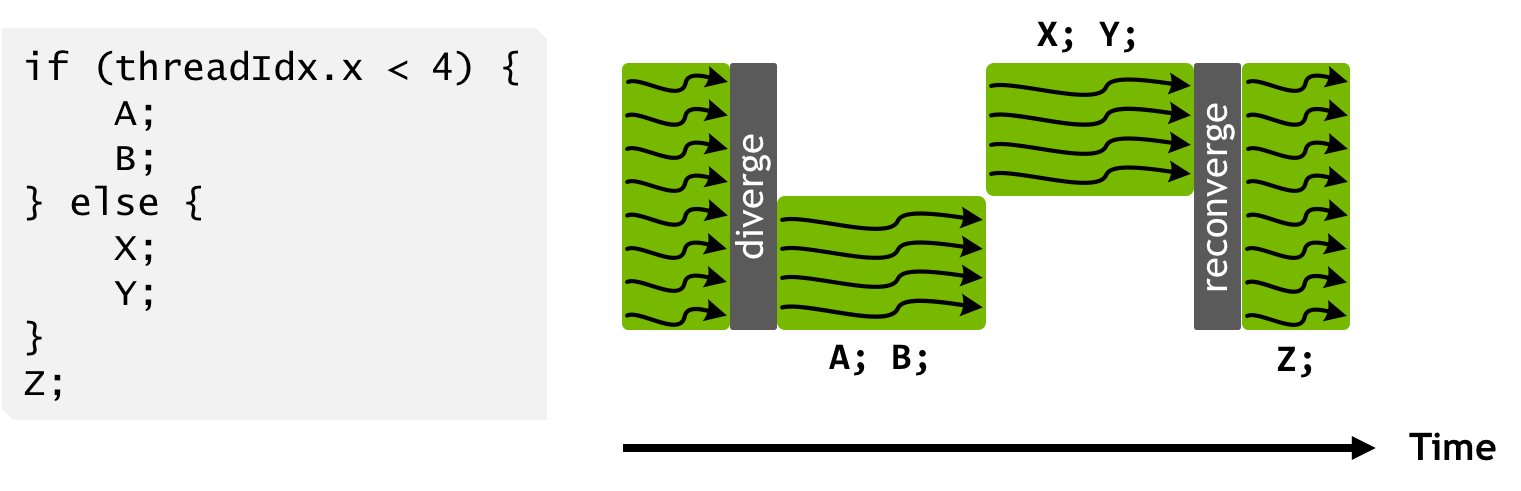
\includegraphics[width=0.8\textwidth]{cuda_thread_divergence_old.png}
	\caption{Branching in device \citep{site:cuda}.}
	\label{fig:thread_divergence_old}
\end{figure}

% TODO: Maybe mention global memory access

On the surface, the device code is very similar to the host code written for the CPU, and will most likely work correctly if written as if for the CPU. But to maximize performance, one must keep in mind the SIMT model, grouping into warps, thread divergence when branching, coalesced memory accesses etc.

On the other side of the spectrum, the SIMT execution model can be compared to the Single instruction, multiple data (SIMD) execution model, where the number of elements processed by a single instruction is directly exposed in the user code, compared to the SIMT model, where the user code itself describes a behavior of a single thread and the grouping of threads is abstracted by the platform. 

\subsection{Thread hierarchy}

Apart from being grouped into warps, threads on the device are also grouped into Cooperative Thread Arrays (CTA), also known as thread blocks. Thread blocks can be one-dimensional, two-dimensional or three-dimensional, which provides an easy way for work distribution when processing arrays, matrices or volumes. Thread blocks are further organized into one-dimensional, two-dimensional or three-dimensional grid, as can be seen in Figure \ref{fig:thread_hierarchy}. When launching a kernel, we specify thread block size and grid size, which combined together give us the number of threads executing the given kernel.

\begin{figure}[h]
	\centering
	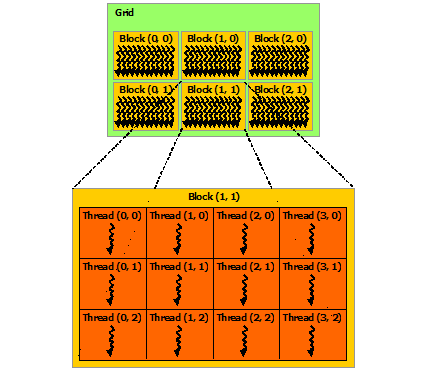
\includegraphics[width=0.8\textwidth]{grid_of_thread_blocks.png}
	\caption{Thread grouping hierarchy \citep{site:cuda}.}
	\label{fig:thread_hierarchy}
\end{figure}

Each thread is assigned an index, accessible through \texttt{threadIdx} built-in variable. Each thread can also access the index of the thread block it is part of through \texttt{blockIdx}, the block size through \texttt{blockDim} and grid size through \texttt{gridDim}. All of these variables are three dimensional vectors, with dimensions unused during kernel launch set to zero for indices and one for dimensions. Using these built-in variables, we can distribute work between threads, most often assigning each thread a part of the input to process.

\subsection{Thread cooperation}
\label{sec:thread_cooperation}
CUDA provides several mechanisms for thread cooperation. Threads can cooperate on the following levels of thread hierarchy, with increasing speed and capability:

\begin{itemize}
	\item grid level,
	\item thread block level,
	\item warp level.
\end{itemize}

The rest of this subsection describes the older API using intrinsic functions. The newer Cooperative Groups API, which is a superset of the older API, is described in the subsection \ref{sec:cooperative_groups}.

\subsubsection{Grid level}
On grid level, the only available tools for cooperation are atomic operations on global memory. These operations can be used to perform read-modify-write on a 32-bit or 64-bit word in global memory without introducing race conditions.

\subsubsection{Thread block level}
On a thread block level, threads can use two mechanisms for cooperation:
\begin{itemize}
	\item shared memory,
	\item synchronization barrier.
\end{itemize}

As per the CUDA C++ programming guide: 
"the shared memory is expected to be a low-latency memory near each processor core (much like an L1 cache) and \_\_syncthreads() is expected to be lightweight" \citep{site:cuda}.

Shared memory is a small on-chip memory, described in more detail in the subsection \ref{sec:memory_hierarchy}. Each thread block has private shared memory, accessible only from threads of the given thread block. Shared memory can be used as software managed cache or to share results between threads of the thread block. 

To synchronize access to shared memory between threads of the thread block, we use synchronization barrier \texttt{\_\_syncthreads()}. All threads in the block must execute the call to \texttt{\_\_syncthreads()} before any of the threads can proceed beyond the call to \texttt{\_\_syncthreads()}. 
The \texttt{\_\_syncthreads()} function also serves as memory barrier. % TODO: Maybe describe what memory barrier is

\subsubsection{Warp level}
% TODO: Describe masks for all the functions
On warp level, threads of the warp, or lanes as they are referred to in the documentation, can utilize intrinsic functions to exchange data without the use of shared memory and perform simple hardware accelerated operations. For operations, warps can perform:
\begin{itemize}
	\item reduce-and-broadcast operations,
	\item broadcast-and-compare operations,
	\item reduce operations,
\end{itemize}

% This is important as this is the basis of one of our algorithms
For data exchange, CUDA C++ provides several warp shuffle instructions. There are four source-lane addressing modes:
\begin{itemize}
	\item direct lane index,
	\item copy from lane with ID lower by \textit{delta},
	\item copy from lane with ID higher by \textit{delta},
	\item copy from lane based on bitwise XOR of provided \textit{laneMask} and own lane ID. 
\end{itemize}

The data exchange does not have to span the whole warp. Shuffle operations allow the warp to be subdivided into groups with width of any power of 2.

Only direct lane indexing performs lane index wrap around. If the given lane index is out of the range $[0:width - 1]$, the actual lane index is computed as $srcLane \mod width$. In other addressing modes, the lanes with out of range source lane index are left unchanged, receiving the value they pass in. The wrap around mechanism allows us to rotate data between threads instead of just shifting. The direct lane indexing can also be used to broadcast a value from a single lane to all other lanes. % TODO: Maybe mention how the wrap around can be used to implement ring buffer shifting between two parts of a buffer

For warp level operations, the reduce-and-broadcast operations receive a single integer value from each lane which they compare to zero, making it effectively a boolean. The results of the comparison are then reduced in one of the following ways and the result is broadcast to all threads:
\begin{itemize}
	\item result is non-zero if and only if all of the values are non-zero,
	\item result is non-zero if any of the values are non-zero,
	\item result contains single bit for each lane which is set if the value given by the lane was non-zero
\end{itemize}

The broadcast-and-compare operations broadcast the value given by each lane and compare it to the value given by the current lane, returning:
\begin{itemize}
	\item mask of lanes that have the same value,
	\item mask if all threads in mask gave the same value, 0 otherwise.
\end{itemize}

Finally, there are the general reduce operations. \textit{Add}, \textit{min}, \textit{max} operations are implemented for signed or unsigned integer values. \textit{And}, \textit{or}, \textit{xor} operations are implemented for unsigned integers only.

The API described in this subsection forms the basis of thread cooperation in CUDA. Most of this API is available since the early versions of CUDA. Subsection \ref{sec:cooperative_groups} will describe a newer Cooperative groups API, which builds on top of and extends the API described in this subsection.

\subsection{Cooperative groups}
\label{sec:cooperative_groups}

Cooperative Groups API, introduced with CUDA 9, is an extension to the CUDA programming model for organizing groups of communicating threads \citep{site:cuda}. The API introduces data types representing groups of cooperating threads, be it a warp, a part of a warp, a thread block, a grid or even a multigrid (representing multiple grids each running on a separate device). 


The API distinguishes two types of groups. First are the \textit{implicit groups}, which are present implicitly in each CUDA kernel. These are:

\begin{itemize}
	\item thread block,
	\item grid,
	\item multigrid.
\end{itemize}

The API provides functions for the creation of handles for data types representing the implicit groups. 

The other type are \textit{explicit groups}, which must be explicitly created from one of the implicit groups. 

\begin{itemize}
	\item thread block tile,
	\item coalesced group.
\end{itemize}

Both of these groups represent warp or subwarp size grouping of threads. Thread block tile can be created from a thread block or from other thread block tile, representing a warp or a part of a warp of size of a power of 2. The warp level operations described in the previous subsection \ref{sec:thread_cooperation} are available as methods on this group, with mask and width arguments of the built-in functions implicitly derived from the properties of the group. 

% TODO: Explaing coalesced group


Creating a handle for an implicit group is a collective operation, in which all threads of the group must participate. Creating the group handle in a conditional branch may lead to deadlocks or data corruption. It may also introduce unnecessary synchronization points, limiting concurrency. Similarly to implicit group handle creation, partitioning of groups is a collective operation which must be executed by all threads of the parent group and may introduce synchronization points. It is recommended to create implicit group handles and do all partitioning at the start of the kernel and pass const references throughout the code \cite{site:cuda}.

\subsection{Memory hierarchy}
\label{sec:memory_hierarchy}

Each CUDA device has its own DRAM memory, so called \textit{device memory} or \textit{VRAM} in GPU properties, separate from the host system memory and from the \textit{device memory} of all other devices. Physically, \textit{device memory} can be seen on most GPU boards as DRAM chips separate from the main silicon chip.

Data has to be transferred from or to the \textit{device memory} over the PCI-e bus, either explicitly by calls to \textit{cudaMemcpy} or by mapping parts of host memory to the \textit{device memory} address space using the \textit{Unified Memory} system, which then handles the data transfers in the background automatically.

From the point of view of a CUDA thread, there are several types of memory available, as can be seen on Figure \ref{fig:memory_types}. For this thesis, the main types are:

\begin{itemize}
	\item local memory,
	\item shared memory,
	\item global memory,
	\item registers.
\end{itemize}

\begin{figure}[h]
	\centering
	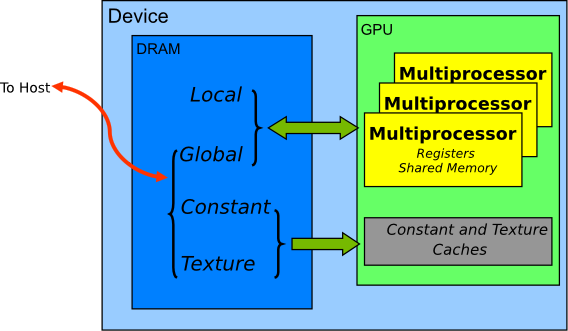
\includegraphics[width=0.8\textwidth]{memory-spaces-on-cuda-device.png}
	\caption{Memory types on a CUDA device \citep{site:cuda}.}
	\label{fig:memory_types}
\end{figure}

Local and global memory are both allocated from device memory, and as such have very high access latency. 

\textbf{Local memory} is private for each thread, allocated automatically based on the requirements of the CUDA compiler. This type of memory is used for register spilling, arrays with non-constant indexing and large structures or arrays which would consume too much register space. 

\textbf{Global memory} is shared by all threads of a kernel, and as such any access which could lead to race condition must be synchronized using atomic operations, as described in Section \ref{sec:thread_cooperation}. Global memory is allocated by the host code using \texttt{cudaMalloc} family of functions. When host code transfers data to the device using \texttt{cudaMemcpy} or any other means, global memory is the part of device memory this data will reside in. The pointers returned by \texttt{cudaMalloc} and possibly used in \texttt{cudaMemcpy} are then passed as arguments to the kernel. Device code can then use these to access the global memory. 

\textbf{Shared memory}, as mentioned in the section \ref{sec:thread_cooperation}, is expected to be a low-latency memory near each processor core (much like an L1 cache). The relation with L1 cache can be seen in the fact that each kernel can configure the proportion between hardware allocated to L1 cache and to Shared memory, which means these memories share the same underlying hardware. Shared memory can be allocated either dynamically by declaring an array type variable with the memory space specifier \texttt{\_\_shared\_\_} and providing the size to be allocated during kernel launch, or statically by defining the variable with static size.


\textbf{Registers} are the fastest memory available. Compared to CPUs, GPUs provide large amount of registers. For all recent GPU generations, the register file provides 65536 32bit registers. 

\subsection{Streaming multiprocessor}
\label{sec:sm}
NVIDIA GPUs are build around an array of \textit{Streaming multiprocessors} (SM). SM of a GPU is similar to a core of a multicore CPU. Each SM has separate execution units, schedulers, register file, shared memory and L1 cache. An example of an SM can be seen in Figure \ref{fig:volta_sm}. Each SM can have multiple schedulers, each scheduling up to one warp per cycle. 

Each thread block is assigned to a single SM exclusively, and each SM can run multiple thread blocks at once. Warps of all thread blocks resident on the given SM are scheduled regardless of the thread block the warps belong to.

% TODO: More

\begin{figure}[h]
	\centering
	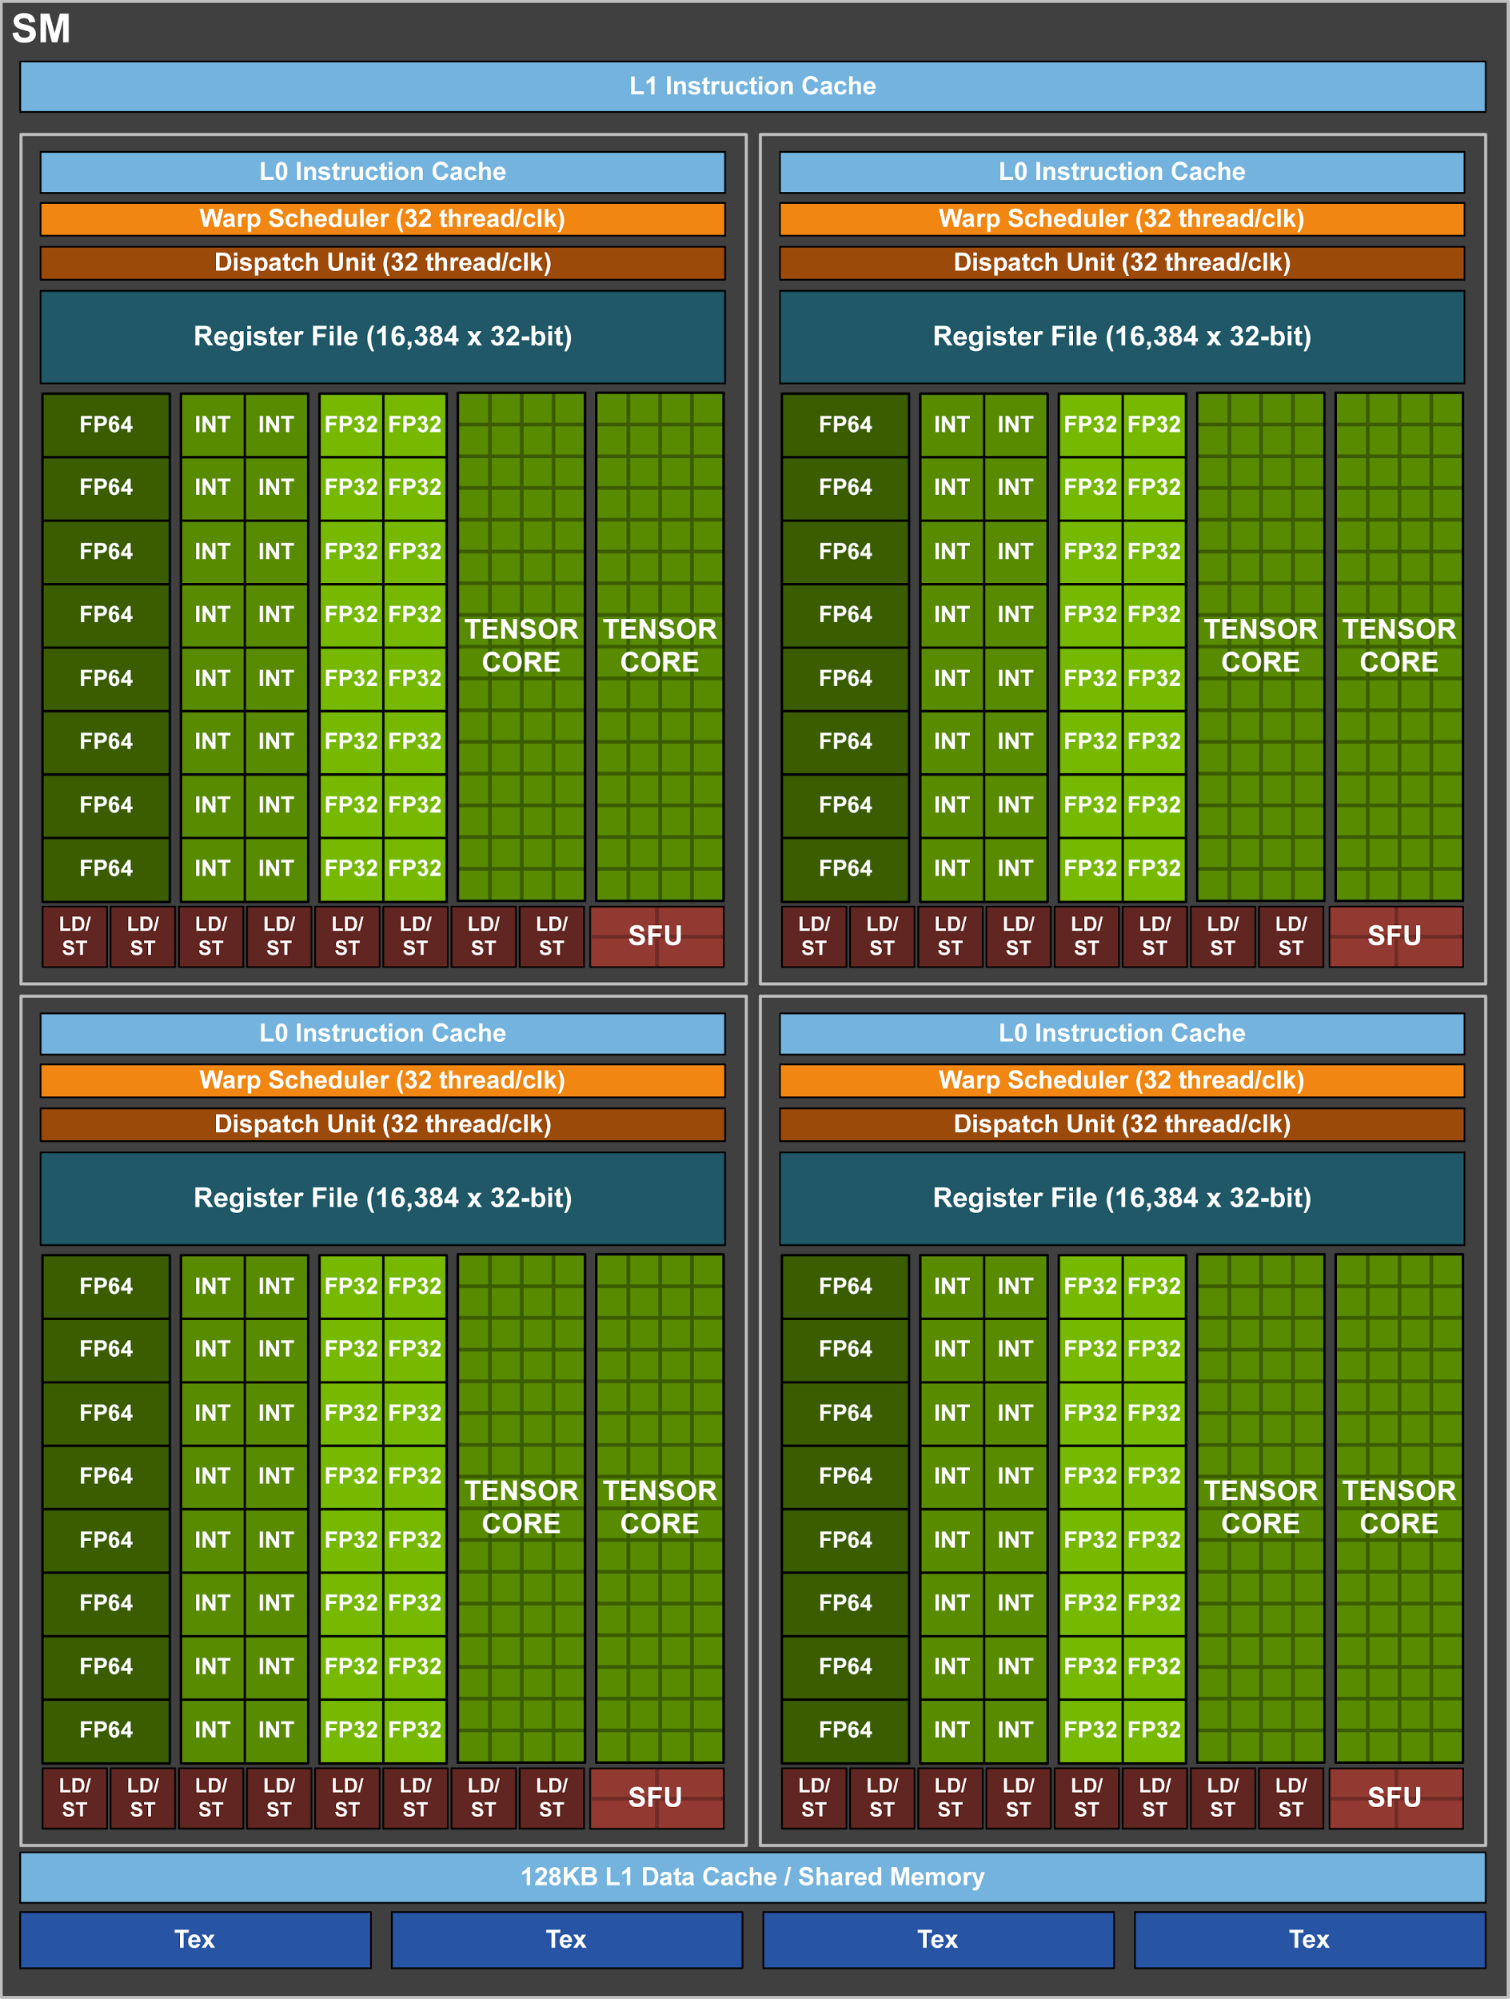
\includegraphics[width=0.8\textwidth]{volta_sm.png}
	\caption{Streaming multiprocessor \citep{paper:volta}.}
	\label{fig:volta_sm}
\end{figure}

\subsection{Versioning}

When working with CUDA, there are two main parts of the platform which are versioned separately: % TODO: Add driver version
\begin{itemize}
	\item CUDA Toolkit,
	\item GPU Compute Capability.
\end{itemize}

CUDA Toolkit represents the software development part of the CUDA platform, encompassing the CUDA runtime library, the \textit{nvcc} compiler and other tools for development of the software.

GPU Compute Capability (CC) represents the features provided by the hardware. This includes the number of registers, memory sizes, set of instructions and other features. In general, each consumer GPU generation corresponds to a new CC, such as GTX 1000 cards corresponding to CC 6.0 Pascal and RTX 3000 cards corresponding to CC 8.0 Ampere. There are some exceptions, for example CC 7.0 Volta having only enterprise cards. With each release of new Compute Capability cards, there is generally accompanying CUDA Toolkit release providing access to the new features provided by the hardware. Compute Capabilities are backwards compatible, so code created for older generation of cards can be ran on newer cards, even though it may not take advantage of new hardware features and may be inefficient on the newer cards.

\section{Code optimizations}

This section introduces basic principles for producing performant CUDA code.
The observations and recommendations provided in this section are based on the principles and properties described in the previous section \ref{sec:programming_model}.

\subsection{Occupancy}

The GPU design prioritizes high instruction throughput of many concurrent threads over single thread performance at the cost of high latency of each instruction. To hide the high latency between dependent instructions, each scheduler keeps a pool of warps between which it switches, possibly on each instruction. Warps in a pool of a scheduler are called \textit{active} warps.
Each cycle, there may be multiple warps which have instructions ready to be executed. Such warps are called \textit{eligible} warps.
Each cycle, a warp scheduler can select one of the \textit{eligible} warps as \textit{issued} warp, issuing its instruction to be executed.

For optimal performance, we want to have enough active warps so that there is at least one eligible warp each cycle to enable the GPU to hide the high latency of each instruction. As described in Section \ref{sec:sm}, the number of warps resident on a SM depends on the number and size of thread blocks resident on a SM.

The number of thread blocks assigned to an SM is limited by three factors:

\begin{itemize}
	\item hardware limit,
	\item register usage,
	\item shared memory usage.
\end{itemize}

The hardware limit differs, but is either 16 or 32 for all currently supported Compute Capabilities. 

To enable no cost execution context (program counters, registers, etc.) switching, the whole execution context for all warps is kept on-chip for the whole lifetime of each warp. 


Number of registers used by all warps of all blocks which reside on the given SM must be smaller than or equal to the number of registers in the register file. For example, for SM with 65536 registers, code using 64 registers per thread and 512 threads in a block, there can only be two blocks resident on the SM, as $2*512*64 = 65536$. If the code requires only a single register more, only a single block will be resident on each SM.

The total amount of shared memory required by all blocks residing on an SM must be smaller than or equal to the size of shared memory provided by the SM. 

\subsection{Pipeline saturation}

Other than occupancy, there are other possible reasons why no warp may be eligible in a given cycle. Pipeline saturation is one of such reasons. GPU hardware has several pipelines, each implementing a different part of the instruction set. As an example, for the RTX 2060 card, these include:
\begin{itemize}
	\item Load Store Unit (LSU),
	\item Arithmetic Logic Unit (ALU),
	\item Fused Multiply Add/Accumulate (FMA),
	\item Transcendental and Data Type Conversion Unit (XU).
\end{itemize}

Each instruction has a Compute Capability specific throughput, which if exceeded makes the pipeline implementing the instruction saturated and unable to execute any other instructions. This becomes a problem when, for example, many or all warps often execute the same low throughput instruction, such as sinus, cosinus or inverse square root, which are implemented by the XU pipeline. Even for simpler operations implemented by the ALU or FMA, if all warps execute the same instruction, the pipelines may become saturated and warps which are waiting to execute more of the given instruction will not be eligible to be issued.

High LSU utilization reflects that the program may be memory bound, waiting for data from global or shared memory, or that the program executes many warp shuffle instructions, which are also implemented by the LSU pipeline. Due to this, the usage of shared memory together with warp shuffles is not advisable, as they both utilize the same pipeline and compete for resources.

% TODO: Maybe screenshot from NSIGHT Compute

\subsection{Global memory access}

As we can see in Figure \ref{fig:global_memory_access}, the access to global memory is grouped into 128~B naturally aligned chunks, where any chunk accessed by any of the threads of the warp has to be transferred from slow global memory. The maximum performance is achieved when access to memory is aligned and coalesced, i.e. all threads of a warp access 32 consecutive 32bit elements of an array which are aligned to 128~B. Any other form of access introduces overhead in a form of unnecessary data being transferred from memory. 

\begin{figure}[h]
	\centering
	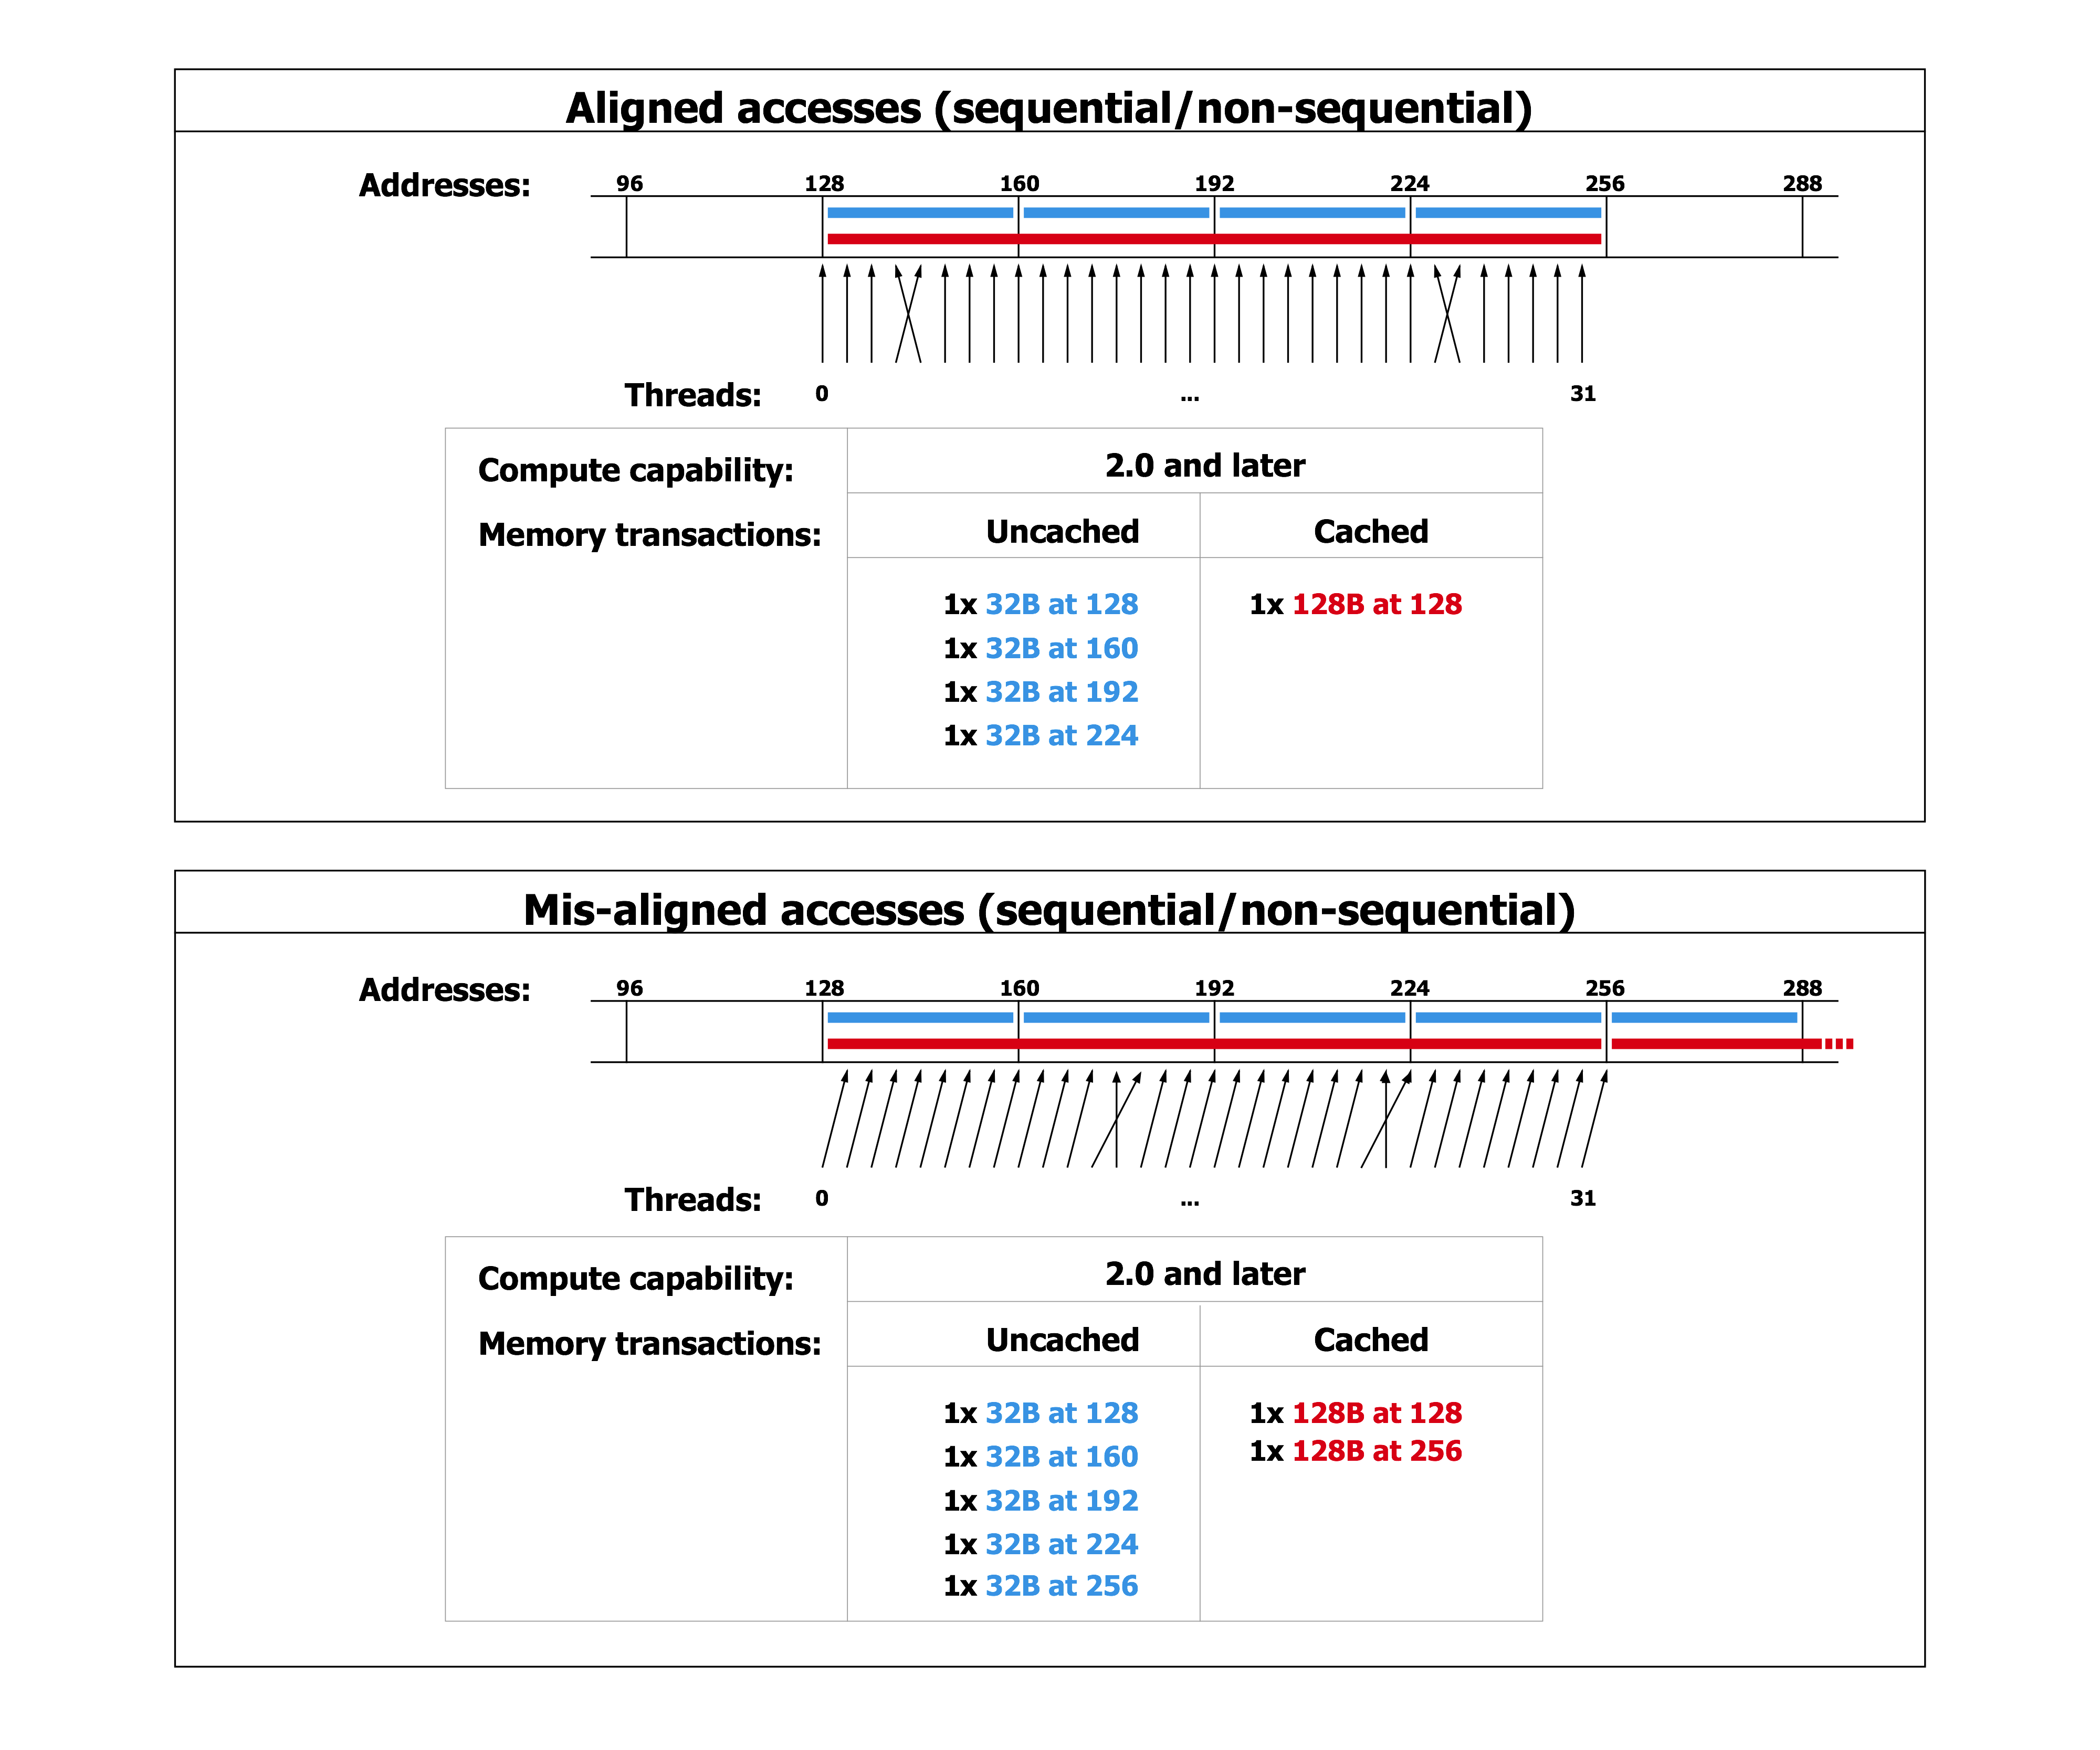
\includegraphics[width=0.8\textwidth]{global-memory-access.png}
	\caption{Global memory access \citep{site:cuda}.}
	\label{fig:global_memory_access}
\end{figure}

\subsection{Shared memory access}
To achieve high bandwidth, shared memory is divided into 32 banks. The optimal access pattern shared memory is designed for is that each thread of a warp accesses a different bank. To enable this access pattern, successive 32bit words are mapped to successive shared memory banks. The simplest pattern is that the 32 threads of a warp access 32 successive 32bit items from an array in shared memory, as can be see in the left column of Figure \ref{fig:shared_memory_access}. If multiple threads access different addresses mapping to the same bank, as can be seen in the middle column of the figure, their accesses are serialized, the throughput being divided by the maximum number of different addresses accessed in any of the banks. This is called a \textit{bank conflict}. Access to a the same address by multiple threads does not lead to a bank conflict, broadcasting the value between the threads instead.

\begin{figure}[h]
	\centering
	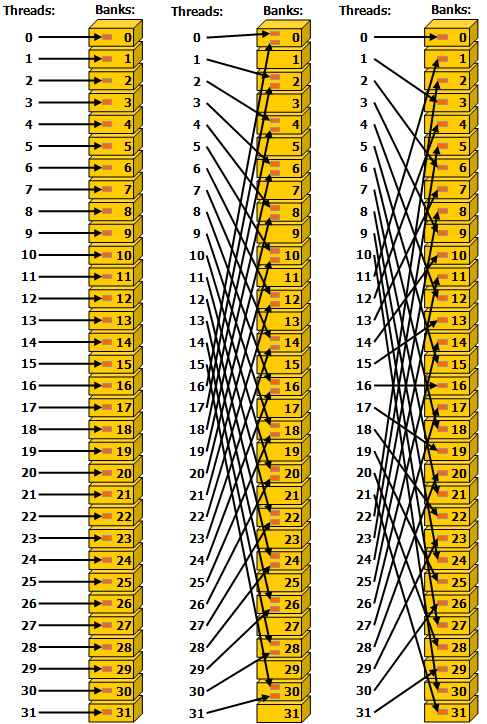
\includegraphics[width=0.8\textwidth]{shared-memory-access.png}
	\caption{Shared memory access patterns \citep{site:cuda}.}
	\label{fig:shared_memory_access}
\end{figure}

\subsection{General recommendations}

We can summarize the information in previous subsections into few simple rules \citep{site:cuda}:

\begin{enumerate}
	\item Maximize parallel execution to achieve maximum utilization;
	\item Optimize memory usage to achieve maximum memory throughput;
	\item Optimize instruction usage to achieve maximum instruction throughput.
\end{enumerate}

To maximize parallel execution, ensure that the workload is distributed between large enough number of threads, where each thread requires low enough number of registers and each thread block requires small enough part of shared memory so that as many as possible fit onto an SM.

To optimize memory usage, minimize transfers from lower bandwidth memory by reusing data in hardware cache or manually move data to shared memory. When accessing global memory, utilize coalesced accesses to minimize unnecessary data transferred. When accessing shared memory, minimize bank conflicts.

To optimize instruction usage, minimize the use of low throughput instructions such as sinus, cosinus or inverse square root. When working with floating point numbers, use 32 bit numbers if precision is not crucial. Minimize thread divergence to ensure all threads in a warp execute useful instructions.

% TODO: Move related work to Analysis chapter
%\section{Related work}

% Accelerating Radio Astronomy Cross-Correlation with Graphics Processing Units

% Kapinchev GPU Implementation of Cross-Correlation for Image Generation in Real Time






\section{Goals}

The goal of this thesis is to measure and quantify the effectiveness of optimizations for different cross-correlation usage patterns. The main objective is to compare the effectiveness of the implementation using Fast Fourier transform and the naive algorithm and measure the input size on which the effectiveness of FFT overtakes the the naive algorithm.

Secondary goal is to optimize the naive implementation from the thesis by \citep{misko}, describe any deficiencies in the original code and quantify the gains when these deficiencies are corrected.

\chapter{Implementation}

In this chapter, we first give a high level overview of the possibilities for parallelization and data reuse in the implementation of definition-based cross-correlation algorithm, introduced in section \ref{sec:cross_corr_def}. Next we describe several such implementations.


The definition-based algorithm has several properties which allow for parallelization, optimization through data reuse and distribution of work.

Figure \ref{fig:cross_corr_shifts} depicts the output matrix with corresponding relative shift of the two input matrices for each element. As described in Section \ref{sec:cross_corr_opt}, each of these elements can be computed independently in parallel.

Each overlap defines a unique set of element pairs which are to be multiplied. Each pair of overlapping elements is uniquely assigned to a single shift of the two matrices. 

\begin{figure}[h]
	\centering
	\def\svgwidth{\textwidth}
	% Must be relative to current directory
	% as input ignores graphicspath, which is
	% only for includegraphics{}
	\input{./img/overlap-Shifts.pdf_tex}
	\caption{Result matrix with corresponding relative shifts.}
	\label{fig:cross_corr_shifts}
\end{figure}


\section{Parallelization}
In this section, we first reformulate the definition-based cross-correlation algorithm into the language of independent parallel tasks, then we define the types of workers which can be derived from CUDA Thread hierarchy, described in Section \ref{sec:thread_hierarchy}. Next we introduce the possible distributions of tasks between different types workers, with options for data reuse and load balancing.

\subsection{Two matrices}
When we focus on the computation of cross-correlation between two matrices, called one-to-one in the rest of the thesis, we can reformulate the definition-based algorithm as a problem with two levels of independent parallel tasks, as can be seen in Figure \ref{fig:cross_corr_one_to_one_tasks}. First level are the different relative shifts of the two input matrices, each represented by a single element in the output matrix. Each of these tasks has a set of independent subtasks corresponding to overlapping pairs of elements of the two input matrices. Each subtask is depicted as a yellow square in Figure \ref{fig:cross_corr_one_to_one_tasks}. Each of these subtasks belongs to exactly one set. The results of all subtasks in a set have to be summed into the result of the parent task. The set of subtasks defines a continuous submatrix in both input matrices.

\begin{figure}[h]
	\centering
	\def\svgwidth{\textwidth}
	% Must be relative to current directory
	% as input ignores graphicspath, which is
	% only for includegraphics{}
	\input{./img/overlap-Tasks.pdf_tex}
	\caption{Tasks hierarchy in definition-based one-to-one cross-correlation.}
	\label{fig:cross_corr_one_to_one_tasks}
\end{figure}

The goal is to distribute the subtasks between workers in such a way that we maximize parallelism, maximize data reuse and minimize the need for communication and synchronization between workers.

\subsection{Many matrices}

With more than two matrices, we can add additional levels to the task hierarchy shown in \ref{fig:cross_corr_one_to_one_tasks}. As described in Section \ref{sec:cross_corr_forms}, there are several forms of cross-correlation between multiple matrices can be computed. These are:
\begin{enumerate}
	\item \textit{one-to-many},
	\item \textit{n-to-mn},
	\item \textit{n-to-m}.
\end{enumerate}

As we can see, the \textit{one-to-one} type, described in the previous section, together with the \textit{one-to-many} type, are subtypes of the more general \textit{n-to-mn} type. We separate the \textit{one-to-one} and \textit{one-to-many} types as they offer a great possibility for caching the single matrix for use in all computations.

All of the described types can be partitioned into many \textit{one-to-one} cross-correlations, as can be seen in Figure \ref{fig:cross_corr_many_tasks}. For both \textit{n-to-mn} and \textit{n-to-m} types, the number of green top level tasks, corresponding to the number of result matrices, is equal to $n*m$. To reiterate, the difference between these two types is that in the \textit{n-to-mn} type, each of the \textit{n} left matrices is cross-correlated with a different set of \textit{m} right matrices.

\begin{figure}[h]
	\centering
	\def\svgwidth{0.8\textwidth}
	% Must be relative to current directory
	% as input ignores graphicspath, which is
	% only for includegraphics{}
	\input{./img/overlap-ManyTasks.pdf_tex}
	\caption{Task hierarchy of types with many matrices.}
	\label{fig:cross_corr_many_tasks}
\end{figure}

As in the case of \textit{one-to-one} type, the meaning of the boxes is as follows:

\begin{itemize}
	\item Each green box represents a pair of input matrices, or equivalently a single output matrix;
	\item Each orange box represents an element in the result matrix, or equivalently a relative shift of the two input matrices;
	\item Each yellow box represents a pair of overlapping elements from the two input matrices.
\end{itemize}

All boxes on a given level can be processed completely independently. Results of the children of an orange box have to be summed together. Results of the children of a green box have to be written into a single matrix in memory, each into a different element without any collisions.

% TODO: Segway to data reuse

\subsection{CUDA workers}

Section \ref{sec:thread_hierarchy} described how CUDA threads are hierarchically grouped from smallest to largest as follows:

\begin{enumerate}
	\item thread,
	\item warp,
	\item thread block,
	\item grid.
\end{enumerate}

This thesis provides several implementations of the definition-based cross-correlation algorithm described in following sections, each mapping different level of task hierarchy shown in Figure \ref{fig:cross_corr_many_tasks} to different size of CUDA thread group.

Based on the choice of the CUDA thread group size, we can use smaller groups to compute the subtree of the assigned task, and primitives provided by larger groups to synchronize, communicate and combine results of the tasks between different workers.

\section{Warp shuffle algorithm}

This section describes the implementation of definition-based cross-correlation built on Warp Shuffle instructions. We first introduce a simple version of the implementation, later improving it step by step until we arrive at the algorithm actually implemented in the code accompanying this thesis.

Warp shuffle instruction are utilized to shift data loaded from the left matrix and broadcast data loaded from the right matrix between threads in a warp. CUDA threads are used as workers, with tasks representing a single relative shift of the two matrices (which is equivalent to a single element in the output matrix), as can be seen in Figure \ref{fig:warp_shuffle_simple_tasks}.

\begin{figure}[h]
	\centering
	\def\svgwidth{0.8\textwidth}
	% Must be relative to current directory
	% as input ignores graphicspath, which is
	% only for includegraphics{}
	\input{./img/overlap-WarpShuffleSimpleTasks.pdf_tex}
	\caption{Tasks in simple warp shuffle algorithm.}
	\label{fig:warp_shuffle_simple_tasks}
\end{figure}

The main idea behind this algorithm is illustrated in Figure \ref{fig:warp_shuffle_shuffle}. Threads of a single warp process 32 consecutive shifts in the \textit{x} axis all with the same \textit{y} axis value, as can be seen in Figure \ref{fig:warp_shuffle_simple_dist}. Figure \ref{fig:warp_shuffle_shuffle} shows how two neighboring threads process elements of the two input matrices. The numbers represent iterations of a \textit{for loop} in the code. 

\begin{figure}[h]
	\centering
	\def\svgwidth{0.8\textwidth}
	% Must be relative to current directory
	% as input ignores graphicspath, which is
	% only for includegraphics{}
	\input{./img/overlap-WarpShuffleShuffle.pdf_tex}
	\caption{Work done by two neighboring threads.}
	\label{fig:warp_shuffle_shuffle}
\end{figure}

As can be seen, the element from the left matrix processed by thread \textit{t} in iteration \textit{k} is required by thread \textit{t - 1} in iteration \textit{k + 1}. This holds for all threads of a warp and maps exactly onto the Warp Shuffle Down function, described in Section \ref{sec:thread_cooperation}. 


In any given iteration, all threads of a warp require the exact same element
from the right matrix. This broadcast can be implemented using the general Warp Shuffle function with direct source lane indexing.

The problem of iteration \textit{3}, in which the lower thread does not have any value to compute, can be solved in several ways. If we were programming for a CPU, we would give the two for loops implementing the two worker threads different bounds so that the second worker stops earlier. More GPU friendly implementation needs to prevent thread divergence of a warp by executing the range check for each thread only once when loading the data from the left matrix into a register of the thread. If the thread is loading value outside the matrix, it loads 0 instead. This makes the result of the multiplication 0 which is then added to the sum, making it a \textit{noop} and preventing thread divergence.

% TODO: Distribution of shifts between threads and blocks, block dimensions etc.

\begin{figure}[h]
	\centering
	\def\svgwidth{0.8\textwidth}
	% Must be relative to current directory
	% as input ignores graphicspath, which is
	% only for includegraphics{}
	\input{./img/overlap-WarpShuffleWarps.pdf_tex}
	\caption{Distribution of shifts between CUDA threads, warps and blocks.}
	\label{fig:warp_shuffle_simple_dist}
\end{figure}

% TODO: Top and bottom parts of the left buffer

The final algorithm can be described by the following pseudocode:

\begin{lstlisting}[
style=cuda
]

float sum = 0;
for (
	size_t warp_y_right = warp_right_start.y; 
	warp_y_right < warp_right_end.y;
	++warp_y_right 
) {
	size_t warp_y_left = warp_y_right + warp_min_shift.y;
	
	
}
\end{lstlisting}



\subsection{Work distribution}

In the simplified algorithm described above, there are massive differences in work done by different threads. As we can see in Figure \ref{fig:warp_shuffle_work_difference}, the thread processing the left overlap has much less work than the thread processing the right overlap. This will lead to problems with occupancy once the threads with small amount of work are completed. 

\begin{figure}[h]
	\centering
	\def\svgwidth{0.6\textwidth}
	% Must be relative to current directory
	% as input ignores graphicspath, which is
	% only for includegraphics{}
	\input{./img/overlap-WarpShuffleWorkDifference.pdf_tex}
	\caption{Task size difference in the simplified algorithm.}
	\label{fig:warp_shuffle_work_difference}
\end{figure}

To distribute the work more evenly, we need to change what is considered a task processed by a worker. Compared to the simplified implementation, , task represents several full continuous rows of overlapping pairs of elements (yellow boxes), as can be seen in figure \ref{fig:warp_shuffle_work_dist_tasks}. With this change, multiple workers may write to the same element in the output matrix. Each worker must add the final sum of the assigned tasks to sums of all other workers processing tasks of the same shift. As each worker needs to add the sum just once, utilizing the \textit{atomicAdd} operation on the output matrix in global memory is sufficient. The maximum number of rows in a task is provided as an argument to the algorithm, and influences the number of workers created.

\begin{figure}[h]
	\centering
	\def\svgwidth{0.8\textwidth}
	% Must be relative to current directory
	% as input ignores graphicspath, which is
	% only for includegraphics{}
	\input{./img/overlap-WarpShuffleWorkDistTasks.pdf_tex}
	\caption{Tasks in warp shuffle algorithm with load balancing.}
	\label{fig:warp_shuffle_work_dist_tasks}
\end{figure}


We provide several algorithms to derive the number of workers started and the distribution of tasks between workers from the provided argument and the size of the input. The provided algorithms are:

\begin{itemize}
	\item None,
	\item Rectangle,
	\item Triangle.
\end{itemize}


The algorithms are illustrated in Figures \ref{fig:work_dist_max_1} and \ref{fig:work_dist_max_2}. In these, the purple boxes represent number of tasks for each shift in the given row of the output matrix. As we can see in Figure \ref{fig:worker_id_assignment}, the worker ID is shared by all threads with the same rank in the \textit{x} axis. This means that worker ID is assigned based on the \textit{y} axis rank of each thread and is shared by all threads of a warp. 

The \textit{None} distribution is provided mainly to measure the overhead of the code changes required to implement work distribution. This distribution behaves identically as the simplified algorithm with no distribution.

The \textit{Rectangle} distribution computes the maximum number of tasks required for any shift, and starts this maximum number of workers for all shifts, creating a rectangle of workers as can be seen in Figure \ref{fig:work_dist_max_1}. The worker API is designed to stop workers which are not required, stopping the redundant workers immediately after work assignment. The tasks are assigned using simple modulo operati


The \textit{Triangle} distribution starts exactly one worker for each task. The disadvantage of this distribution is the complex computation required to assign worker to task. This computation includes many multiplications, divisions and most importantly a low throughput square root instruction. For small inputs where the size of tasks is small, the overhead of triangle distribution may be greater than any gains provided by work distribution. 
% TODO: Image why is it called triangle

The total number of workers started for given number of tasks can be seen in Figures \ref{fig:work_dist_max_1} and \ref{fig:work_dist_max_2}. The first figure shows maximum work distribution, with each worker processing exactly one row of input. The second figure shows the same inputs, but with each worker processing at most 2 rows.

\begin{figure}[h]
	\centering
	\def\svgwidth{\textwidth}
	% Must be relative to current directory
	% as input ignores graphicspath, which is
	% only for includegraphics{}
	\input{./img/overlap-DistMax1Row.pdf_tex}
	\caption{Work distribution of 4x4 input with 1 row per task.}
	\label{fig:work_dist_max_1}
\end{figure}


\begin{figure}[h]
	\centering
	\def\svgwidth{\textwidth}
	% Must be relative to current directory
	% as input ignores graphicspath, which is
	% only for includegraphics{}
	\input{./img/overlap-DistMax2Rows.pdf_tex}
	\caption{Work distribution of 4x4 input with maximum of 2 rows per task.}
	\label{fig:work_dist_max_2}
\end{figure}

This algorithm modifies the number of blocks started for each kernel. In the simplified algorithm, block size is configurable, but is pretty much static. The \textit{x} axis size of a block is used to simplify grouping threads into warp, and as such has a hardcoded size of 32. The \textit{y} axis size of a block is used to configure number of warps per block, and is provided as an argument to the algorithm. The number of blocks is then chosen to cover the output matrix in both \textit{x} and \textit{y} axes with one thread per output matrix element, with some possible overallocation due to the difference between size of the output matrix and the preset size of the block.


This algorithm retains the same size of a block and use of the \textit{x} axis of grid size. As all threads with the same value of \textit{x} axis always process the same rows, we only need to multiply the number of workers by using the \textit{y} axis of the grid size to start the number of workers required by given work distribution algorithm. 

Again, all threads with the same \textit{x} axis thread rank (combination of the \textit{x} axis of the thread block and the \textit{x} axis of the thread itself) have the same \texttt{worker\_id}, and us such all either run the same rows or end if the worker they represent is redundant. This can be seen in Figure \ref{fig:worker_id_assignment}.



\subsection{Improving ratio of arithmetic instructions}
\label{sec:arith_ratio}

% TODO: Describe that the multiplication and addition are computed as fused multiply-add operation
Another problem of the simplified implementation, shared with the work distributing implementation, is the ratio of warp shuffle instructions to arithmetic instructions. For each multiplication of the pair of input values, represented by a single yellow box, and addition of this result to the total sum, we must execute three warp shuffle instructions. This makes warp shuffle instructions the bottleneck in these implementations, as can be seen in Figure \ref{fig:warp_shuffle_shuffle_profiling}. We can also see that the multiplication and addition are implemented as fused multiply-add (FMA) instruction. 

There are several ways to improve the ratio of warp shuffle instructions to arithmetic instructions. The simplest one is to utilize the \textit{one-to-many} type of computation, and let single worker compute cross-correlation between one left matrix and many right matrices at once. This first allows data reuse, as the data from the left matrix is loaded only once to be used to compute multiple results. The second advantage is that we only need a single additional warp shuffle for each additional right matrix, which also adds a single multiplication and addition. The ratio of warp shuffles to fused multiply-add operations can then be expressed as $2 + r : r$, which is much improved from the $3:1$ ratio of the simplified warp shuffle algorithm.

% TODO: Profiling
The effects of this optimization can be seen when we compare Figure \ref{fig:warp_shuffle_profiling_original} with Figure \ref{fig:warp_shuffle_profiling_multiple_right}. %TODO: Describe

% Why is it important that the arrays are in registers
This optimization heavily relies on


More complex version of this optimization is to process multiple rows from the same right matrix, which can be used to improve the ration even for \textit{one-to-one} type of computation. There are several caveats when implementing this optimization. The main difference is that a single thread now computes multiple different shifts instead of the same shift in multiple matrices. These shifts differ in the \textit{y} axis, and represent consecutive elements in a column of the output matrix. Each of these shifts represents different overlap of the two input matrices, requiring different bounds in the \textit{y} axis. % TODO: Image

Due to these different bounds for the shifts computed by each thread, we have to add explicit initialization and finalization code which handles the case where only some of the rows of the right matrix overlap with given row from the left matrix. % TODO: Image


The complexity of the code forces us to share the results of different function calls, such as the initialization, main body and finalization, through shared memory. We allocate a shared memory array to with maximum number of shifts per thread times the number of threads per block, which is used to accumulate the final result of the computation of all shifts for all threads of the thread block. % TODO: Image of the shared memory array distribution

After the initialization phase is finished, the main loop is conceptually very similar with the multiple right matrices case described previously. The only major differences are the accumulation of the final result through shared memory instead of through registers and the reversal of the results for given row group   % TODO: Why is it reversed, IMAGE



% https://forums.developer.nvidia.com/t/loop-through-register-array-without-using-local-memory/29458/3
\subsection{Problems with local memory}

The optimizations described in the previous section \ref{sec:arith_ratio} hint at further possibilities, such as using multiple left matrices and multiple rows from the left matrix in combination with the previous optimizations. The problem we encountered is that these additional changes lead to much more complex indexing which the \textit{nvcc} compiler cannot expand into static compile time indexing, even though logically we can see it is. % TODO: Code samples

This leads to compiler pulling the \texttt{thread\_right}, \texttt{thread\_left\_top}, \texttt{thread\_left\_bottom} and \texttt{sum} to be allocated from local memory instead of from register file. The change from local memory results in a substantial overhead, which can be seen in Figure \ref{fig:local_memory_impact}. 



\section{Occupancy improvement}

For small inputs, processing a single shift or even just several rows per thread may not start enough threads and lead to low occupancy.  
% TODO: Shift per warp
% TODO: Why not block per warp




\chapter{Results}
\label{sec:results}

In this chapter, we first describe our setup for measurement and validation of the implementations described in the previous chapter. We then compare the definition-based cross-correlation implementations against each other before comparing them with an FFT-based CUDA implementation. Finally, we compare the definition-based implementations with existing real-world cross-correlation implementations in the Python SciPy library and in Matlab.

\section{Experiments}
\label{sec:experiments}
As the main aim of this thesis is to compare implementations of an algorithm, the code is heavily instrumented to enable measurements and comparisons of different parts of the implementation. This instrumentation is designed to limit its impact and to allow measurements that minimize background noise and imprecision of the time measurement tools provided by the CUDA C++ language.

As part of this thesis, we have also developed a benchmarking tool that allows the use of a declarative description of the set of benchmarks to be executed. The tool generates input and validation data, runs the benchmarks for all inputs and with all argument combinations specified, and records the times and validation results. As such, the tool is used both for measurements and for validation of the implementation. 

To simplify the implementation of the definition-based algorithm optimizations, we have placed several restrictions on the input matrices and the computation:
\begin{itemize}
	\item both input matrices are of the same size,
	\item whole output matrix is computed.
	% TODO: If I do not manage to finish it in time, this should be fixed and expanded
\end{itemize}

Both restrictions are used to simplify the implementation and reduce the number of variables when measuring. Both restrictions could be removed in production-grade implementation but would make the optimizations unnecessarily harder to implement. 

\subsection{Code instrumentation}
\label{sec:code_instrumentation}

All implementations, including definition-based, FFT-based, and CPU-based, are split into the following steps:

\begin{itemize}
	\item \textit{Load} loads the input matrices into host memory,
	\item \textit{Prepare} allocates device memory and precomputes things derived from the input data size,
	\item \textit{Transfer} moves data from host to device memory,
	\item \textit{Run} executes the computation,
	\item \textit{Finalize} moves data from device to host memory,
	\item \textit{Free} releases resources allocated in the \textit{Prepare} step,
	\item \textit{Store} stores results from host memory.
\end{itemize}

Each of these steps can be individually measured and compared. The main focus of this thesis is the \textit{Run} step, but to properly compare the behavior of the FFT-based implementations with definition-based implementations, we will have to compare other steps as well.

We also provide simple CPU-based single-threaded definition-based implementation, for which most of these steps are empty. This implementation is provided for the basic validation of results and of the benchmarking infrastructure. 


The code instrumentation allows us to measure the algorithms with three different levels of granularity:
\begin{itemize}
	\item \textit{Compute} measuring the duration of the Prepare, Transfer, Run, Finalize, and Free steps together;
	\item \textit{CommonSteps} measuring every step separately;
	\item \textit{Algorithm} measuring algorithm-specific parts such as individual kernels or library calls.
\end{itemize}

For parts that can be executed repeatedly, such as computations and data transfers, we utilize measurement with an adaptive iteration count. The number of iterations is automatically increased until the measured duration is longer than a configured minimum, most often a second. This type of measurement should mitigate background noise and get around problems with minimum clock resolution for very short steps. It is used for the \textit{Compute} measurement, for measuring the \textit{Run} step, and for measuring kernel and function call durations in each algorithm.

For timing the SciPy implementation, we use the \texttt{perf\_counter\_ns} function provided by the Python standard library. For Matlab, the pair of functions named \texttt{tic} and \texttt{toc} is used to measure the execution time. For both implementations, we also utilize the adaptive iteration count. For both, we measure with only the \textit{Compute} granularity.


\subsection{Experiment setup}

Experiments were run on two systems:
\begin{itemize}
	\item Intel Xeon Silver 4110 with 256GB of RAM and NVIDIA Tesla V100 PCIe 16 GB (gpulab), running Rocky Linux 8.5, gcc 11.2, CUDA 11.6, and nvidia driver 510.47.03;
	\item AMD Ryzen 5 4600H with 16GB of RAM and NVIDIA GeForce RTX 2060 (laptop), running Ubuntu 20.04, gcc 9.4.0, CUDA 11.4, and nvidia driver 470.129.06.
\end{itemize}

The two systems allow us to evaluate our implementations on two different classes of GPU hardware, gpulab representing the enterprise server systems with Tesla GPU and Xeon CPU, and laptop representing consumer hardware with gaming GeForce card and Ryzen CPU. The two systems also allow us to compare two different GPU generations, Compute Capability 7.0 for the V100 and Compute capability 7.5 for the RTX 2060. Unless stated otherwise, the results showcased in this text are measured on gpulab. Laptop results will be added only when the behavior significantly differs from that of gpulab, as the algorithms are in no way optimized for any of the two cards and should run similarly in both cases. 

Most showcased results are collected using the adaptive iteration count. The timing is done using CUDA events when measuring the run time of CUDA kernels or the high-resolution clock provided by the C++ standard library for all other measurements. The resulting value shown is the total measured time divided by the number of iterations. To further remove noise, all measurements are repeated 20 times, and the mean of these measurements is taken as the final result, as there are no significant outliers that would skew the mean.



\subsection{Result validation}


When validating the results of a computation, we compare them to valid results computed using SciPy, Matlab, or our simple CPU definition-based implementation. The output matrix is compared element by element with the valid result, computing a matrix of differences using formula \ref{eq:result_comparison} \citep{wiki:relative_difference}.

% See https://en.wikipedia.org/wiki/Relative_change_and_difference
% and https://c-faq.com/fp/fpequal.html
\begin{equation}
\label{eq:result_comparison}
\mathrm{Relative\_difference }(a, b) = \frac{\abs{a - b}}{\max(\abs{a}, \abs{b})}
\end{equation}

The maximum element in the matrix of differences is then taken as the error of the output matrix.

\section{Comparing definition-based algorithms}
\label{sec:results_definition_based}

In this section, we first measure and compare the members of the Warp shuffle algorithm family, described in Section \ref{sec:warp_shuffle_alg}, against each other. Next, we compare the members of the Warp per shift algorithm family, introduced in Section \ref{sec:warp_per_shift}. Lastly, we compare the best optimizations from both algorithm families with the Basic definition-based implementation.


Each of the \textit{one-to-one}, \textit{one-to-many}, \textit{n-to-mn}, and \textit{n-to-m} input types is compared separately, as it allows for different optimizations and may benefit certain implementations better than others. In the following sections, we list and use only the best-performing arguments for each implementation. The benchmarks measuring behavior with different argument values which were used to choose these optimal arguments are available in the thesis attachments in the directory \texttt{code/benchmarking/args\_test}. The results were left out of the text of the thesis for brevity, as they closely follow the descriptions of each optimization.  

When comparing the definition-based algorithms, we measure only the kernels in the \textit{Run} step, as the implementation of this step is the only difference between the algorithms. As such, the speedup reported in this section represents only the change in execution time of the \textit{Run} step, i.e., the computation itself, not including allocations, loading from disk, transfers to GPU, etc.

Implementations utilizing warp shuffle instructions are usable across a range of input sizes. We measure their behavior for input matrix sizes ranging from 16x16 to 512x512 elements. These input matrix sizes were chosen as the larger input sizes are faster computed using the FFT-based implementation, and as such the speed of the optimizations of the definition-based implementation is irrelevant for the larger sizes. Based on the input type, we also measure with a different number of left and right input matrices to gauge the changes in the behavior of the implementations with a changing number of input matrices.


\subsection{Warp shuffle optimizations with the one-to-one input}
\label{sec:results_warp_shuffle_one_to_one}
For this input type, we have the following four implementations with these arguments:

\begin{center}
	\begin{tabular}{|l|l|c|} 
		\hline
		Implementation&Argument&Value\\ [0.5ex] 
		\hline\hline
		Simple & Warps per thread block & 4 \\
		\hline
 		\multirow{3}*{Simple with work distribution} & Warps per thread block & 8\\
 		\cline{2-3}
 		& Rows per thread & 1 \\
 		\cline{2-3}
 		& Distribution type & triangle \\
 		\hline
 		\multirow{2}*{Multirow right} & Warps per thread block & 4\\
 		\cline{2-3}
 		& Right rows per thread & 8\\
 		\hline
 		\multirow{3}*{Multirow both} & Warps per thread block & 4\\
 		\cline{2-3}
 		& Shifts per thread & 8\\
 		\cline{2-3}
 		& Left rows per iteration & 4\\
		\hline
	\end{tabular}
\end{center}

\begin{figure}[ht]
	\centering	
	\begin{subfigure}{0.4\textwidth}
		\centering
		\def\svgwidth{\textwidth}
		% Must be relative to current directory
		% as input ignores graphicspath, which is
		% only for includegraphics{}
		\input{./img/warp_shuffle_one_to_one_gpulab.pdf_tex}
		\caption{gpulab}
		\label{fig:warp_shuffle_one_to_one_results_gpulab}
	\end{subfigure}
	\begin{subfigure}{0.4\textwidth}
		\centering
		\def\svgwidth{\textwidth}
		% Must be relative to current directory
		% as input ignores graphicspath, which is
		% only for includegraphics{}
		\input{./img/warp_shuffle_one_to_one.pdf_tex}
		\caption{laptop}
		\label{fig:warp_shuffle_one_to_one_results_laptop}
	\end{subfigure}

	
	\caption{Speedup of \textit{one-to-one} warp shuffle optimizations.}
	\label{fig:warp_shuffle_one_to_one_results}
\end{figure}

The results displayed in Figure \ref{fig:warp_shuffle_one_to_one_results} show the speedup of each optimization compared to the Simple warp shuffle implementation. For smaller inputs on gpulab, the \textit{multirow} optimizations are slower, up to 31\% slower for the \textit{multirow\_both} and up to 68\% slower for the \textit{multirow\_right} than the Simple implementation. This slowdown is caused by the reduction in the number of threads and correspondingly reduced occupancy of the GPU. Due to the smaller size of the laptop GPU, the reduced number of threads has a much lower effect. For \textit{multirow\_right}, this is combined with each thread reading each row of the right input matrix multiple times, adding global memory access latency, which the GPU is unable to hide due to the low occupancy. This problem is mitigated in the \textit{multirow\_both} optimization, which is reflected here in better performance for all input sizes when compared with the \textit{multirow\_right} optimization. For larger input sizes, the better ratio of warp shuffle to fused multiply-add instructions of these two optimizations allows them to overtake the Simple implementation. This is above 128x128 for \textit{multirow\_both} and above 320x320 for \textit{multirow\_right} on gpulab. For laptop, the lower performance of the GPU increases the effect of the optimizations, overtaking the Simple implementation sooner. 

The behavior of work distribution optimization tells us that the gpulab GPU is not fully saturated by the Simple implementation up until the 320x320 input matrix size. Again due to the smaller size of the laptop GPU, it is saturated much sooner. Low occupancy is an expected problem with the \textit{one-to-one} input type. On gpulab for inputs smaller than 320x320, the large number of additional threads allows us to fully utilize the GPU, making the work distribution optimization more than four times faster than the Simple implementation without work distribution for certain input matrix sizes. As we increase the input size, the benefit of additional threads diminishes, completely disappearing above 320x320 input size, where the overhead introduced by the additional threads negates the increased GPU saturation. 

The maximum absolute time improvement is for the 512x512 input size, improving from $67.18$~ms to $24.08$~ms on gpulab and from $303$~ms to $72$~ms on laptop.
% Make just one diagram showing the four implementations and their behavior across the input sizes
% Mention the optimal arguments used


\subsection{Warp shuffle optimizations with the one-to-many input}
This input type has six implementations with the following arguments:

\begin{center}
	\begin{tabular}{|l|l|c|} 
		\hline
		Implementation&Argument&Value\\ [0.5ex] 
		\hline\hline
		Simple & Warps per thread block & 4 \\
		\hline
		\multirow{2}*{Multimat right} & Warps per thread block & 4 \\
 		\cline{2-3}
 		& Right matrices per thread & 8 \\
		\hline
		\multirow{4}*{Multimat right with work distribution} & Warps per thread block & 8 \\
		\cline{2-3}
		& Right matrices per thread & 8 \\
		\cline{2-3}
		& Rows per thread & 1 \\
		\cline{2-3}
		& Distribution type & triangle \\
		\hline
		\multirow{3}*{Multirow right multimat right} & Warps per thread block & 4 \\
		\cline{2-3}
		& Right rows per thread & 2 \\
		\cline{2-3}
		& Right matrices per thread & 4 \\
		\hline
		\multirow{4}*{Multirow both multimat right} & Warps per thread block & 4 \\
		\cline{2-3}
		& Shifts per right matrix & 4 \\
		\cline{2-3}
		& Right matrices per thread & 4 \\
		\cline{2-3}
		& Left rows per iteration & 4 \\
		\hline
	\end{tabular}
\end{center}

\begin{figure}[ht]
	\centering	
	\begin{subfigure}{0.4\textwidth}
		\centering
		\def\svgwidth{\textwidth}
		\input{./img/warp_shuffle_one_to_many_2_matrices_gpulab.pdf_tex}
		%\label{fig:executed_instructions_shared_mem}
	\end{subfigure}
	\begin{subfigure}{0.4\textwidth}
		\centering
		\def\svgwidth{\textwidth}
		\input{./img/warp_shuffle_one_to_many_8_matrices_gpulab.pdf_tex}
		%\label{fig:pipeline_utilization_shared_mem}
	\end{subfigure}
	\hfill
	\begin{subfigure}{0.4\textwidth}
		\centering
		\def\svgwidth{\textwidth}
		\input{./img/warp_shuffle_one_to_many_16_matrices_gpulab.pdf_tex}
		%\label{fig:executed_instructions_shared_mem}
	\end{subfigure}
	\begin{subfigure}{0.4\textwidth}
		\centering
		\def\svgwidth{\textwidth}
		\input{./img/warp_shuffle_one_to_many_1024_matrices_gpulab.pdf_tex}
		%\label{fig:pipeline_utilization_shared_mem}
	\end{subfigure}
	
	\caption{Speedup of \textit{one-to-many} warp shuffle optimizations on gpulab.}
	\label{fig:warp_shuffle_one_to_many_results}
\end{figure}

\begin{figure}[ht]
	\centering	
	\begin{subfigure}{0.4\textwidth}
		\centering
		\def\svgwidth{\textwidth}
		\input{./img/warp_shuffle_one_to_many_8_matrices_gpulab.pdf_tex}
		\caption{gpulab}
		\label{fig:warp_shuffle_one_to_many_results_gpulab}
	\end{subfigure}
	\begin{subfigure}{0.4\textwidth}
		\centering
		\def\svgwidth{\textwidth}
		\input{./img/warp_shuffle_one_to_many_8_matrices.pdf_tex}
		\caption{laptop}
		\label{fig:warp_shuffle_one_to_many_results_laptop}
	\end{subfigure}
	
	\caption{Comparison of the input with 8 right matrices on gpulab and laptop.}
	\label{fig:warp_shuffle_one_to_many_results_gpulab_vs_laptop}
\end{figure}

From the results in Figure \ref{fig:warp_shuffle_one_to_many_results}, we see that most optimizations are more than 50\% slower than the Simple implementation for small input sizes and small numbers of matrices. This is caused by lower occupancy of the GPU, as both \textit{multimat} and \textit{multirow} group multiple overlaps into each job, reducing the total number of jobs and decreasing the total number of workers. The exception is \textit{Multimat right with work distribution}, where the \textit{work distribution} optimization is specifically designed to solve the problem of low occupancy by splitting each overlap into several jobs. This results in the 4 times speedup we see for the input 32x32 with two right input matrices. However, with increasing total input size, be it the size of each matrix or the total number of matrices, the need to increase occupancy diminishes, and the speedup provided by \textit{work distribution} is lower.

For larger input sizes, the improved ratio of warp shuffle instructions to fused multiply-add instructions balances out the decreased occupancy. The combination of \textit{multimat right} and \textit{multirow right} is slightly better than the \textit{multimat right} optimization alone but is hampered by the increased number of reads from global memory as each row from the right input matrix is reread two times by each worker. This is also the reason why the argument \textit{right rows per thread} is best when set to 2, as increasing the value of this argument increases the number of times each row is read by the given worker. This is the reason why for larger inputs, the \textit{multimat right} and its combination with \textit{multirow right} provide similar speedup, as any improvement of the instruction ratio is balanced by the increased number of reads.

The best improvement for the input sizes we are interested in is provided by the combination of \textit{multimat right} with \textit{multirow both}. This combination removes the disadvantage of multiple reads of the \textit{multirow right}, leaving just the improved instruction ratio.

When we compare behavior on gpulab and laptop in Figure \ref{fig:warp_shuffle_one_to_many_results_gpulab_vs_laptop}, we see that the change is very similar to the one shown in Section \ref{sec:results_warp_shuffle_one_to_one}. The optimizations improving occupancy are not as effective, while the optimizations reducing the number of warp shuffle instructions and global memory accesses significantly improve the performance. The measurement in Figure \ref{fig:warp_shuffle_one_to_many_results_laptop}, computing input with 8 right matrices, are very similar to the results from Figure \ref{fig:warp_shuffle_one_to_many_results} with 16 input matrices, i.e., with twice the input data size. This shows the effects of the lower performance and smaller size of the GPU.

The maximum absolute improvement is for the $512 \times 512$ matrix size with 1024 right matrices, where we see a decrease from $67$~s to $16.8$~s on gpulab and from $308$~s to $67$~s on laptop.

\subsection{Warp shuffle optimizations with the n-to-mn input}
This input type shares implementations with the \textit{one-to-many} type, as it does not provide any additional possibilities for data reuse because each left input matrix is cross-correlated with a different set of $m$ right input matrices. This means that each implementation of \textit{n-to-mn} type just executes the \textit{one-to-many} implementation kernel $n$ times in parallel, once for each left input matrix. Due to this, the main factor here is how many of the \textit{one-to-many} kernels can we run in parallel, or more precisely, how many thread blocks from these kernels can fit on a single SM.

The arguments differ slightly due to the higher GPU utilization:

\begin{center}
	\begin{tabular}{|l|l|c|} 
		\hline
		Implementation&Argument&Value\\ [0.5ex] 
		\hline\hline
		Simple & Warps per thread block & 4 \\
		\hline
		\multirow{3}*{Simple with work distribution} & Warps per thread block & 4 \\
		\cline{2-3}
		& Rows per thread & 1 \\
		\cline{2-3}
		& Distribution type & triangle \\
		\hline
		\multirow{2}*{Multimat right} & Warps per thread block & 4 \\
		\cline{2-3}
		& Right matrices per thread & 8 \\
		\hline
		\multirow{4}*{Multimat right with work distribution} & Warps per thread block & 4 \\
		\cline{2-3}
		& Right matrices per thread & 8 \\
		\cline{2-3}
		& Rows per thread & 1 \\
		\cline{2-3}
		& Distribution type & triangle \\
		\hline
		\multirow{4}*{Multirow right multimat right} & Warps per thread block & 4 \\
		\cline{2-3}
		& Right rows per thread & 2 \\
		\cline{2-3}
		& Right matrices per thread & 4 \\
		\cline{2-3}
		& Number of CUDA streams & 16 \\
		\hline
		\multirow{5}*{Multirow both multimat right} & Warps per thread block & 4 \\
		\cline{2-3}
		& Shifts per right matrix & 4 \\
		\cline{2-3}
		& Right matrices per thread & 4 \\
		\cline{2-3}
		& Left rows per iteration & 4 \\
		\cline{2-3}
		& Number of CUDA streams & 16 \\
		\hline
	\end{tabular}
\end{center}

\begin{figure}[ht]
	\centering	
	\begin{subfigure}{0.4\textwidth}
		\centering
		\def\svgwidth{\textwidth}
		\input{./img/warp_shuffle_n_to_mn_2_4_gpulab.pdf_tex}
		%\label{fig:executed_instructions_shared_mem}
	\end{subfigure}
	\begin{subfigure}{0.4\textwidth}
		\centering
		\def\svgwidth{\textwidth}
		\input{./img/warp_shuffle_n_to_mn_4_16_gpulab.pdf_tex}
		%\label{fig:pipeline_utilization_shared_mem}
	\end{subfigure}
	\hfill
	\begin{subfigure}{0.4\textwidth}
		\centering
		\def\svgwidth{\textwidth}
		\input{./img/warp_shuffle_n_to_mn_100_1000_gpulab.pdf_tex}
		%\label{fig:executed_instructions_shared_mem}
	\end{subfigure}
	
	\caption{Speedup of \textit{n-to-mn} warp shuffle optimizations on gpulab.}
	\label{fig:warp_shuffle_n_to_mn_results}
\end{figure}

These measurements are very similar to the measurements for the \textit{one-to-many} type. The differences in measurements between the same implementation used in these two input types reflect the total resources required by the kernel, i.e., how many kernels can run in parallel.


The results in Figure \ref{fig:warp_shuffle_n_to_mn_results} show that for a small number of small input matrices, the \textit{work distribution} optimization is still necessary to balance out the occupancy reduced by other optimizations. The arguments of the implementations using \textit{work distribution} are optimized for the smallest input sizes. To run with the same arguments for input matrices of size 512x512 would require the CUDA grid size of 65536 in the \textit{y} axis, which is just above the 65535 maximum limit. The same implementations did run for the 512x512 input size in \textit{one-to-many} as they were run with eight warps per thread block, which reduces the required grid size, and for \textit{one-to-many} was faster than four warps per thread block. In the measurements for \textit{n-to-mn} type, the version with four warps per thread block came out faster. 
As work distribution is only faster for the smaller input sizes, we choose to use the four warps per thread even if it cannot run the whole range of input sizes, as we try to optimize the speedup for each size separately.

The explanation of the performance of the \textit{multimat right}, the \textit{multirow right multimat right} and the \textit{multirow both multimat right} optimizations is the same as for the \textit{one-to-many} type, as is the effect of running the benchmarks on gpulab when compared to laptop. The occupancy improving optimizations are less effective, while the efficiency improving optimizations are more effective. 
The maximum absolute improvement is for the $512 \times 512$ matrix size with 100 left matrices to 1000 right matrices, where we see decrease from $65.43$~s to $17.29$~s on gpulab and from $303$~s to $69.49$~s on laptop.


\subsection{Warp shuffle optimizations with the n-to-m input}
The final input type has a group of implementations specifically optimized for this type, the \textit{multimat\_both} optimization and its combinations with other optimizations. We also reuse some \textit{one-to-many} implementations, running them $n$ times in parallel, once for each left input matrix, this time all with the same set of right input matrices.

Again, Figure \ref{fig:warp_shuffle_n_to_m_results} shows that \textit{work distribution} is advantageous for smaller inputs, but is not required for larger inputs. As expected, the \textit{multimat\_both} optimization specifically designed for this input type gives the best performance. For smaller inputs, it is best when combined with \textit{work distribution}. For medium and large inputs, it is best when combined with \textit{multirow\_both} optimization. As \textit{multimat right} improvement does not reuse data from the left input matrices, it falls behind the \textit{multimat\_both}.

The maximum absolute improvement is for the $512 \times 512$ matrix size with 50 left matrices to 50 right matrices, where we see a decrease from $163.95$~s to $31.66$~s on gpulab. For laptop, the input with $512 \times 512$ and 50 left matrices and 50 right matrices does not fit into GPU memory. As such, the maximum absolute improvement is for the size $256 \times 256$ with 50 and 50 matrices, decreasing from $49$~s to $14$~s.

\begin{figure}[ht]
	\centering	
	\begin{subfigure}{0.35\textwidth}
		\centering
		\def\svgwidth{\textwidth}
		\input{./img/warp_shuffle_n_to_m_2_4_gpulab.pdf_tex}
		%\label{fig:executed_instructions_shared_mem}
	\end{subfigure}
	\begin{subfigure}{0.35\textwidth}
		\centering
		\def\svgwidth{\textwidth}
		\input{./img/warp_shuffle_n_to_m_4_16_gpulab.pdf_tex}
		%\label{fig:pipeline_utilization_shared_mem}
	\end{subfigure}
	\hfill
	\begin{subfigure}{0.35\textwidth}
		\centering
		\def\svgwidth{\textwidth}
		\input{./img/warp_shuffle_n_to_m_50_50_gpulab.pdf_tex}
		%\label{fig:executed_instructions_shared_mem}
	\end{subfigure}
	
	\caption{Speedup of \textit{n-to-m} warp shuffle optimizations on gpulab.}
	\label{fig:warp_shuffle_n_to_m_results}
\end{figure}

\begin{center}
	\begin{tabular}{|l|l|c|} 
		\hline
		Implementation&Argument&Value\\ [0.5ex] 
		\hline\hline
		\multirow{2}*{Simple} & Warps per thread block & 4 \\
		\cline{2-3}
		& Number of CUDA streams & 8 \\
		\hline
		\multirow{3}*{Multimat right} & Warps per thread block & 4 \\
		\cline{2-3}
		& Right matrices per thread & 8 \\
		\cline{2-3}
		& Number of CUDA streams & 8 \\
		\hline
		\multirow{5}*{Multimat right with work distribution} & Warps per thread block & 4 \\
		\cline{2-3}
		& Right matrices per thread & 8 \\
		\cline{2-3}
		& Rows per thread & 1 \\
		\cline{2-3}
		& Distribution type & triangle \\
		\cline{2-3}
		& Number of CUDA streams & 8 \\
		\hline
		\multirow{3}*{Multimat both} & Warps per thread block & 4 \\
		\cline{2-3}
		& Left matrices per thread & 4 \\
		\cline{2-3}
		& Right matrices per thread & 4 \\
		\hline
		\multirow{5}*{Multimat both with work distribution} & Warps per thread block & 4 \\
		\cline{2-3}
		& Left matrices per thread & 4 \\
		\cline{2-3}
		& Right matrices per thread & 4 \\		
		\cline{2-3}
		& Rows per thread & 1 \\
		\cline{2-3}
		& Distribution type & triangle \\
		\hline
		\multirow{5}*{Multirow both multimat both} & Warps per thread block & 4 \\
		\cline{2-3}
		& Left matrices per thread & 4 \\
		\cline{2-3}
		& Right matrices per thread & 4 \\		
		\cline{2-3}
		& Shifts per right matrix & 4 \\
		\cline{2-3}
		& Left rows per iteration & 4 \\
		\hline
	\end{tabular}
\end{center}





\subsection{Warp per shift optimizations with the one-to-one inputs}
\label{sec:results_occupancy_improvements}

Occupancy is mainly a concern when working with the \textit{one-to-one} input type and small input matrices. Because of this, we implement the algorithms from this family mostly for the \textit{one-to-one} input type and will compare them only for this input type. 

The following table lists the Warp per shift algorithm family implementations, together with the Block per shift algorithm implementation, with the arguments used for their measurement:

\begin{center}
	\begin{tabular}{|l|l|c|} 
		\hline
		Implementation&Argument&Value\\ [0.5ex] 
		\hline\hline
		Warp per shift & Shifts per thread block & 16 \\
		\hline
		\multirow{3}*{Warp per shift with work distribution} & Shifts per thread block & 8\\
		\cline{2-3}
		& Rows per warp & 10 \\
		\cline{2-3}
		& Distribution type & triangle \\
		\hline
		\multirow{4}*{Warp per shift with shared memory} & Shifts per thread block & 16\\
		\cline{2-3}
		& Shared memory row size & 128\\
		\cline{2-3}
		& Load with stride & True\\
		\cline{2-3}
		& Column group per block & True\\
		\hline
		Block per shift & Block size & 256\\
		\hline
	\end{tabular}
\end{center}

From the results in Figure \ref{fig:warp_per_shift_results}, we see that the base Warp per shift implementation is enough to saturate the GPU. Due to this, the Block per shift algorithm and Work distribution optimization do not improve the run time. While still slower than the base Warp per shift implementation, the increasing speed of work distribution with increasing input size is most likely caused by the increasing size of each job and correspondingly decreasing proportion of the overhead caused by distributing the jobs and collecting the results.

\begin{figure}[ht]
	\centering	
	\begin{subfigure}{0.4\textwidth}
		\centering
		\def\svgwidth{\textwidth}
		% Must be relative to current directory
		% as input ignores graphicspath, which is
		% only for includegraphics{}
		\input{./img/warp_per_shift_one_to_one_gpulab.pdf_tex}
		\caption{gpulab}
		\label{fig:warp_per_shift_results_gpulab}
	\end{subfigure}
	\begin{subfigure}{0.4\textwidth}
		\centering
		\def\svgwidth{\textwidth}
		% Must be relative to current directory
		% as input ignores graphicspath, which is
		% only for includegraphics{}
		\input{./img/warp_per_shift_one_to_one.pdf_tex}
		\caption{laptop}
		\label{fig:warp_per_shift_results_laptop}
	\end{subfigure}
	\caption{Relative speed of warp per shift optimizations.}
	\label{fig:warp_per_shift_results}
\end{figure}

The shared memory optimization is not beneficial for inputs smaller than 64x64, mostly due to adding synchronization overhead between warps of a thread block when loading data into shared memory. For larger input data sizes, the reduced number of global memory accesses gives this optimization an advantage over the base Warp per shift implementation.

The largest absolute improvement in run time is for the $512 \times 512$ input matrix size from $0.158$~s to $0.074$~s.



\subsection{Comparison with Basic algorithm}
\label{sec:comparison_with_basic}

Now that we have compared the optimizations of both families separately, we now compare the best of these optimizations against the Basic definition-based implementation described in Section \ref{sec:basic_alg}. As the implementations still differ only in the GPU kernel, we again compare only the time taken by the Run step.


\begin{figure}[ht]
	\centering	
	\begin{subfigure}{0.4\textwidth}
		\centering
		\def\svgwidth{\textwidth}
		\input{./img/definition_based_speedup_one_to_one_gpulab.pdf_tex}
		\caption{One to one.}
		\label{fig:definition_based_speedup_one_to_one}
	\end{subfigure}
	%\hfill
	\begin{subfigure}{0.4\textwidth}
		\centering
		\def\svgwidth{\textwidth}
		\input{./img/definition_based_speedup_one_to_many_gpulab.pdf_tex}
		\caption{One to many.}
		\label{fig:definition_based_speedup_one_to_many}
	\end{subfigure}
	%\hfill
	\begin{subfigure}{0.4\textwidth}
		\centering
		\def\svgwidth{\textwidth}
		\input{./img/definition_based_speedup_n_to_mn_gpulab.pdf_tex}
		\caption{N to MN.}
		\label{fig:definition_based_speedup_n_to_mn}
	\end{subfigure}
	%\hfill
	\begin{subfigure}{0.4\textwidth}
		\centering
		\def\svgwidth{\textwidth}
		\input{./img/definition_based_speedup_n_to_m_gpulab.pdf_tex}
		\caption{N to M.}
		\label{fig:definition_based_speedup_n_to_m}
	\end{subfigure}
	\caption{Speedup of the best optimized implementation compared to Basic implementation on gpulab.}
	\label{fig:definition_based_speedup}
\end{figure}

Figure \ref{fig:definition_based_speedup} shows the achieved speedup for each of the four input types by the best optimization when compared to the Basic implementation. We see inputs for which our implementations are up to 80 times faster. For large inputs, the speedup is around five times, i.e., the computation requires one-fifth of the time required by the Basic implementation.

For the \textit{one-to-one} input type shown in Figure \ref{fig:definition_based_speedup_one_to_one}, we separate the Warp shuffle and Warp per shift based optimizations. As Warp per shift optimizations are designed to improve occupancy, they are generally only relevant for the \textit{one-to-one} input type, as the total size of input data is not enough to saturate the GPU using Basic implementation and simple Warp shuffle implementation. But as we see in the results, Warp shuffle combined with the \textit{work distribution} optimization is almost as fast as Warp per shift. For inputs larger than 200x200, we see that the occupancy is not a limiting factor and the data reuse provided by Warp shuffle optimizations becomes more relevant. The maximum absolute time improvement is from $0.072$s to $0.024$s. For all following input types, we use only Warp shuffle implementations as they are always better than Warp per shift implementations.

The \textit{one-to-many} input type shown in Figure \ref{fig:definition_based_speedup_one_to_many} of up to 80 times when computing one left matrix against 1024 right matrices of size 32x32, achieving the highest speedup. For smaller matrix sizes, increasing the number of right matrices improves speed, which indicates that the GPU is not fully utilized. For larger matrix sizes, the difference between speedups for the different number of matrices becomes negligible, with all converging around a speedup of 5. This seems to be the speedup of our best implementations when GPU is fully saturated. The maximum absolute time improvement is from $86.21$s to $16.83$s. 

The \textit{n-to-mn} input type shown in Figure \ref{fig:definition_based_speedup_n_to_mn} shows different behavior to the \textit{one-to-many} type. The speedup spike for smaller matrix sizes caused by \textit{work distribution} is also present, but now with the increasing number of matrices we get a smaller speedup. Above matrix size of 200x200, optimizations with improved data reuse become prominent, causing the improving speedup for larger matrix sizes. The maximum absolute time improvement is from $83.42$s to $17.29$s. 

The \textit{n-to-m} input type shown in Figure \ref{fig:definition_based_speedup_n_to_m} shows similar characteristics to the \textit{n-to-mn} type. We again see the \textit{work distribution} spike for small matrix sizes, transitioning to optimizations providing better data reuse. The maximum absolute time improvement is from $203.28$s to $31.66$s.

\begin{figure}[ht]
	\centering	
	\begin{subfigure}{0.4\textwidth}
		\centering
		\def\svgwidth{\textwidth}
		\input{./img/definition_based_speedup_one_to_one_gpulab.pdf_tex}
		\caption{One to one.}
	\end{subfigure}
	\begin{subfigure}{0.4\textwidth}
		\centering
		\def\svgwidth{\textwidth}
		\input{./img/definition_based_speedup_n_to_mn_gpulab.pdf_tex}
		\caption{N to MN.}
	\end{subfigure}
	\caption{Speedup of the best optimized implementation compared to Basic implementation on laptop.}
	\label{fig:definition_based_speedup_laptop}
\end{figure}

Two two input types that show a significant difference between gpulab and laptop are shown in Figure \ref{fig:definition_based_speedup_laptop}. The \textit{one-to-one} type again shows the quick falloff of occupancy improving optimizations, which become slower than ones improving the instruction ratio or memory accesses with input matrix size 64x64. We see a similar effect on the \textit{n-to-mn} type, where the initial spike for small inputs caused by occupancy improving optimizations is completely gone. The maximum absolute time improvement is from $351$s to $69$s.

\section{Comparison with existing implementations}

In this section, we compare the best of our definition-based implementations as measured in Section \ref{sec:results_definition_based}, with existing 2D cross-correlation implementations. First, we make a comparison against the FFT-based CUDA implementation. Next, we take two existing tools/libraries in the form of Python SciPy \citet{journal:scipy} library and Matlab \citep{site:matlab} which implement 2D cross-correlation, and compare them with our definition-based algorithms.

We have chosen the Python SciPy library as a generally used CPU implementation of 2D cross-correlation, and Matlab with Parallel Computing Toolbox for GPU accelerated 2D cross-correlation. Due to licensing limitations, Matlab will only be compared on the RTX 2060 system.

The methods for time measurement of all three implementations are described in Section \ref{sec:code_instrumentation}. For each input size (combination of matrix size and the number of matrices), we choose the fastest implementation provided by this thesis. Generally, for smaller inputs, the implementations with work distribution optimization will be chosen, whereas for larger inputs, the implementations optimizing for efficiency through reduced global memory accesses, improved instruction ratios, etc., will be chosen. The comparison of the definition-based implementations and which of them are the fastest for a given input is presented in Section \ref{sec:results_definition_based}. 

\subsection{FFT-based implementation}
\label{sec:results_fft_based}

The FFT-based implementation used in this thesis is adapted from the one used by \citet{misko}. It uses the cuFFT library for the Fast Fourier Transform and a custom kernel for Hadamard multiplication. 

Before comparing this FFT-based implementation with the definition-based implementations, we first show a few properties of this implementation caused by the use of the Fast Fourier transform in general and of the cuFFT library in particular. First is the dependency between the precise size of the input matrix and computation time. As described in the cuFFT library documentation, cuFFT provides "Algorithms highly optimized for input sizes that can be written in the form $2^{a}*3^{b}*5^{c}*7^{d}$. In general, the smaller the prime factor, the better the performance, i.e., powers of two are fastest." \citep{site:cufft}. From our measurements, we see up to 30\% 
slowdown between the power of two input sizes and input sizes one smaller. 

\begin{figure}[ht]
	\centering
	\def\svgwidth{0.3\textwidth}
	% Must be relative to current directory
	% as input ignores graphicspath, which is
	% only for includegraphics{}
	\input{./img/fft_small_compute_time.pdf_tex}
	\caption{Comparison of FFT-based computation in single and double precision for small inputs.}
	\label{fig:fft_double_faster_compute_time}
\end{figure}

Another feature is illustrated in Figure \ref{fig:fft_double_faster_compute_time}, where we show computation time for inputs smaller than 128x128. From these measurements, we see that the cuFFT library computes inputs with matrix size up to 96x96 faster in double precision than in single precision, even though the double precision version works with twice the amount of data and uses operations with lower throughput. The cause is the \textit{Prepare} step, which allocates device memory and in this implementation runs the \textit{cufftPlan*} functions. Based on our measurements, the \textit{Prepare} step is slower for single precision computation than for double precision. Due to the closed source of the cuFFT library, we can only speculate on the cause, but it is most likely due to some additional precomputation done for the single version. 


\begin{figure}[ht]
	\centering	
	\begin{subfigure}{0.4\textwidth}
		\centering
		\def\svgwidth{\textwidth}
		\input{./img/fft_speedup_one_to_one_gpulab.pdf_tex}
		\caption{One to one.}
		\label{fig:fft_speedup_one_to_one}
	\end{subfigure}
	%\hfill
	\begin{subfigure}{0.4\textwidth}
		\centering
		\def\svgwidth{\textwidth}
		\input{./img/fft_speedup_one_to_many_gpulab.pdf_tex}
		\caption{One to many.}
		\label{fig:fft_speedup_one_to_many}
	\end{subfigure}
	%\hfill
	\begin{subfigure}{0.4\textwidth}
		\centering
		\def\svgwidth{\textwidth}
		\input{./img/fft_speedup_n_to_mn_gpulab.pdf_tex}
		\caption{N to MN.}
		\label{fig:fft_speedup_n_to_mn}
	\end{subfigure}
	%\hfill
	\begin{subfigure}{0.4\textwidth}
		\centering
		\def\svgwidth{\textwidth}
		\input{./img/fft_speedup_n_to_m_gpulab.pdf_tex}
		\caption{N to M.}
		\label{fig:fft_speedup_n_to_m}
	\end{subfigure}
	\caption{Speedup of the Basic definition-based implementation and best definition-based optimized implementation compared to FFT-based implementation on gpulab.}
	\label{fig:fft_speedup}
\end{figure}

When comparing the FFT-based implementation with the definition-based implementations, we are mostly interested in the input matrix size where the definition-based and FFT-based implementations are equal and how that size differs between the Basic algorithm and the best of our optimizations, which we now collectively call the \textit{Optimized} algorithm. We call such matrix size the \textit{equality point}, as it is represented by a point where the graphs of the implementations intersect in the diagram. The \textit{Optimized} implementation is chosen for each input (i.e., a combination of input matrix size and number of input matrices) separately. In this section, we measure the whole computation, including allocation, transfer to the GPU, kernel execution, transfer from the GPU, and deallocation. This is because the FFT-based algorithm differs from the definition-based algorithm in all of these stages. Most importantly, we need to include the overhead of the Prepare step that has a major impact on the total run time as described in the previous paragraph.

First, we measure with the same matrix sizes as in previous sections, as shown in Figure \ref{fig:fft_speedup}. The figure shows the speedup of the Basic and Optimized definition-based algorithm compared to the FFT-based implementation, which is used as a baseline. As described above, cuFFT library used by the FFT-based implementation is optimized for certain input sizes, with powers of two being the fastest. As such, measurements in Figure \ref{fig:fft_speedup} are optimal for the FFT-based implementation. The figure shows an improvement in the position of the equality point for all input types.



The most noticeable change between Basic and Optimized implementation is in the \textit{one-to-one} type, shown in Figure \ref{fig:fft_speedup_one_to_one}. Due to the small input data size, the GPU cannot be fully saturated by the FFT-based implementation. Even though this change is the most noticeable, it is the least important, as the total execution time is very low for all implementations of this input type. 

For the \textit{one-to-many} type in Figure \ref{fig:fft_speedup_one_to_many}, the results again show great improvement for small input data sizes, here represented by small number of right input matrices. For these sizes, the Basic implementation often did not reach the speed of the FFT-based algorithm for any measured input matrix size, whereas the optimized implementation has its equality point above the matrix size of 100x100. For inputs with a large number of right input matrices, we see that the equality point moves to around 64x64 input matrices.

The \textit{n-to-mn} type in Figure \ref{fig:fft_speedup_n_to_mn} again displays great similarity to the \textit{one-to-many} type due to the way it is implemented. The equality points are at similar positions, being slightly below 64x64 for the largest input.

The \textit{n-to-m} type in Figure \ref{fig:fft_speedup_n_to_m} shows surprisingly good performance even for the Basic implementation. For inputs with a small number of matrices, optimized equality points are all above 120x120 matrix size. For inputs with a large number of matrices, the equality point is just below 80x80.


When we compare the behavior between gpulab and laptop, as shown in Figure \ref{fig:fft_speedup_laptop}, we see that the FFT-based implementation suffers massively with low occupancy. For smaller input sizes, we see over 100 times improvement for both the \textit{one-to-one} type and for small number of matrices in the \textit{n-to-mn} type. Once the input size becomes large enough, as shown by the 100 to 1000 input for the \textit{n-to-mn} type, the behavior is very similar to that of gpulab, but with much bigger improvements for smaller input matrix sizes.


\begin{figure}[ht]
	\centering	
	\begin{subfigure}{0.4\textwidth}
		\centering
		\def\svgwidth{\textwidth}
		\input{./img/fft_speedup_one_to_one.pdf_tex}
		\caption{One to one.}
		%\label{fig:fft_speedup_one_to_one}
	\end{subfigure}
	\begin{subfigure}{0.4\textwidth}
		\centering
		\def\svgwidth{\textwidth}
		\input{./img/fft_speedup_n_to_mn.pdf_tex}
		\caption{N to MN.}
		%\label{fig:fft_speedup_n_to_mn}
	\end{subfigure}
	\caption{Speedup of the Basic definition-based implementation and best definition-based optimized implementation compared to FFT-based implementation on laptop.}
	\label{fig:fft_speedup_laptop}
\end{figure}


\begin{figure}[ht]
	\centering	
	\begin{subfigure}{0.4\textwidth}
		\centering
		\def\svgwidth{\textwidth}
		\input{./img/fft_speedup_one_to_one_anti_fft_gpulab.pdf_tex}
		\caption{One to one.}
		\label{fig:fft_speedup_antifft_one_to_one}
	\end{subfigure}
	%\hfill
	\begin{subfigure}{0.4\textwidth}
		\centering
		\def\svgwidth{\textwidth}
		\input{./img/fft_speedup_one_to_many_anti_fft_gpulab.pdf_tex}
		\caption{One to many.}
		\label{fig:fft_speedup_antifft_one_to_many}
	\end{subfigure}
	%\hfill
	\begin{subfigure}{0.4\textwidth}
		\centering
		\def\svgwidth{\textwidth}
		\input{./img/fft_speedup_n_to_mn_anti_fft_gpulab.pdf_tex}
		\caption{N to MN.}
		\label{fig:fft_speedup_antifft_n_to_mn}
	\end{subfigure}
	%\hfill
	\begin{subfigure}{0.4\textwidth}
		\centering
		\def\svgwidth{\textwidth}
		\input{./img/fft_speedup_n_to_m_anti_fft_gpulab.pdf_tex}
		\caption{N to M.}
		\label{fig:fft_speedup_antifft_n_to_m}
	\end{subfigure}
	\caption{Speedup when measured in matrix sizes which are prime numbers.}
	\label{fig:fft_speedup_antifft}
\end{figure}

The second set of results, shown in Figure \ref{fig:fft_speedup_antifft}, changes the matrix sizes for which we measure the implementations. We take the matrix sizes used to measure the original results in Figure \ref{fig:fft_speedup} and find the closest prime number. For example 64x64 becomes 61x61, 128x128 becomes 127x127 and 256x256 becomes 257x257. This should make the FFT-based implementation slower, making the improvements provided by our optimizations of definition-based implementation greater as the definition-based implementation is not that closely dependent on the precise size of the input matrices.

We see a major change in the behavior of \textit{one-to-one} type, shown in Figure \ref{fig:fft_speedup_antifft_one_to_one}. The equality point moves beyond the 256x256 matrix size, and we see two peaks in the improvement as the FFT-based implementation becomes faster for the 127x127 input before slowing down again for the 157x157 matrix size. 

% TODO: Expand this
For other input types, we also see an improvement compared to the previous measurements, even if not as significant as for the \textit{one-to-one} type. The speedup values are better across the board, with equality points moving to larger matrix sizes. A similar change is visible when comparing the two measurements on laptop.

\begin{figure}[ht]
	\centering	

	\begin{subfigure}{0.4\textwidth}
		\centering
		\def\svgwidth{\textwidth}
		\input{./img/fft_startup_one_to_many_gpulab.pdf_tex}
		\caption{One to many.}
		\label{fig:fft_startup_one_to_many}
	\end{subfigure}
	%\hfill
	\begin{subfigure}{0.4\textwidth}
		\centering
		\def\svgwidth{\textwidth}
		\input{./img/fft_startup_n_to_mn_gpulab.pdf_tex}
		\caption{N to MN.}
		\label{fig:fft_startup_n_to_mn}
	\end{subfigure}
	%\hfill
	\begin{subfigure}{0.4\textwidth}
		\centering
		\def\svgwidth{\textwidth}
		\input{./img/fft_startup_n_to_m_gpulab.pdf_tex}
		\caption{N to M.}
		\label{fig:fft_startup_n_to_m}
	\end{subfigure}
	\caption{Speedup of the Basic definition-based implementation and best definition-based optimized implementation compared to FFT-based implementation.}
	\label{fig:fft_startup}
\end{figure}

Due to the many iterations of the algorithm which are measured together, the measured time reflects many repeated computations on the same input data. This results in caches being fully populated and allows the cuFFT library possible internal caching. Figure \ref{fig:fft_startup} shows a measurement of a single iteration which limits or possibly even removes the ability for internal caching in the cuFFT library and populating of any caches, measuring \textit{warm-up performance} instead of \textit{sustainable performance}. This type of measurement better reflects the usual usage of a cross-correlation computing function, as it is not useful to compute cross-correlation for the same input multiple times.

This measurement can only be done for large input sizes, as the background noise when measuring smaller input sizes would make any measured results useless. In Figures \ref{fig:fft_startup_one_to_many} and \ref{fig:fft_startup_n_to_mn} we see that the equality point is around 90x90, which is an improvement compared to previous measurements. This hints at some internal caching done by the cuFFT library between computations. The equality point in Figure \ref{fig:fft_startup_n_to_m} is also improved, now just below 60x60.

\subsection{SciPy}
% Reference Scipy implementation

\begin{figure}[ht]
	\centering	
	\begin{subfigure}{0.4\textwidth}
		\centering
		\def\svgwidth{\textwidth}
		\input{./img/scipy_one_to_one_gpulab.pdf_tex}
		\caption{One to one.}
	\end{subfigure}
	%\hfill
	\begin{subfigure}{0.4\textwidth}
		\centering
		\def\svgwidth{\textwidth}
		\input{./img/scipy_one_to_many_gpulab.pdf_tex}
		\caption{One to many.}
	\end{subfigure}
	%\hfill
	\begin{subfigure}{0.4\textwidth}
		\centering
		\def\svgwidth{\textwidth}
		\input{./img/scipy_n_to_mn_gpulab.pdf_tex}
		\caption{N to MN.}
	\end{subfigure}
	%\hfill
	\begin{subfigure}{0.4\textwidth}
		\centering
		\def\svgwidth{\textwidth}
		\input{./img/scipy_n_to_m_gpulab.pdf_tex}
		\caption{N to M.}
		\label{fig:scipy_n_to_m_gpulab}
	\end{subfigure}
	\caption{Speedup of the best definition-based implementation in this thesis compared to SciPy on gpulab.}
	\label{fig:scipy_speedup_gpulab}
\end{figure}


We compare the best of the implementations provided by this thesis with Scipy in Figure \ref{fig:scipy_speedup_gpulab}. Even though SciPy uses multithreaded FFT-based implementation, for any input with an input matrix size above 8x8, the definition-based CUDA C++ implementation is many times faster. We see the speedup increasing with increasing input size for all input types, showcasing the much higher throughput of the GPU. In terms of speedup, we see the \textit{one-to-one} achieving the lowest speedup due to limited occupancy due to small input size, with all other input types achieving up to $3000$ times speedup for the largest input sizes. In terms of absolute times, which range from $0.13$~s for the \textit{one-to-one} type to $2.03$~s for the \textit{n-to-m} type for SciPy, we see improvement to $0.32$~ms and $0.66$~ms respectively.

One figure that stands out is Figure \ref{fig:scipy_n_to_m_gpulab}, where the maximum speedup is not achieved for the largest input in terms of the number of matrices but for a smaller with 4 to 4 matrices. We also see that the speedup does not increase linearly with increased input matrix size apart from the input with 4 to 4 input matrices. This is caused by the algorithm with \textit{multimat\_both} and work distribution optimizations being the fastest for the small input sizes. Once the GPU is sufficiently saturated, another algorithm, this time with both \textit{multimat\_both} and \textit{multirow\_both} optimizations, achieves the highest speedup, which increases at a different rate than for the first algorithm.

For comparison, we show the \textit{n-to-mn} and \textit{n-to-m} input types measured on laptop in Figure \ref{fig:scipy_speedup}. As expected, the behavior is generally the same as on gpulab, only with a smaller total speedup due to the lower performance of the laptop GPU.

In summary, the results are as expected, with SciPy being faster for the smallest inputs as the latency of data transfer and kernel to and from the GPU and the overhead of kernel start are independent of the data size and will result in a slower total speed of the GPU implementation. For all larger inputs, the generally slow speed of Python and limited parallelism of the CPU results in the GPU CUDA C++ implementation being faster.


\begin{figure}[ht]
	\centering	

	\begin{subfigure}{0.4\textwidth}
		\centering
		\def\svgwidth{\textwidth}
		\input{./img/scipy_n_to_mn.pdf_tex}
		\caption{N to MN.}
	\end{subfigure}
	%\hfill
	\begin{subfigure}{0.4\textwidth}
		\centering
		\def\svgwidth{\textwidth}
		\input{./img/scipy_n_to_m.pdf_tex}
		\caption{N to M.}
	\end{subfigure}
	\caption{Speedup of the best definition-based implementation in this thesis compared to SciPy on laptop.}
	\label{fig:scipy_speedup}
\end{figure}

\subsection{Matlab}
% Reference matlab implementation https://www.mathworks.com/help/signal/ref/xcorr2.html?s_tid=mwa_osa_a

\begin{figure}[ht]
	\centering	
	\begin{subfigure}{0.4\textwidth}
		\centering
		\def\svgwidth{\textwidth}
		\input{./img/matlab_one_to_one.pdf_tex}
		\caption{One to one.}
		\label{fig:matlab_one_to_one}
	\end{subfigure}
	%\hfill
	\begin{subfigure}{0.4\textwidth}
		\centering
		\def\svgwidth{\textwidth}
		\input{./img/matlab_one_to_many.pdf_tex}
		\caption{One to many.}
	\end{subfigure}
	%\hfill
	\begin{subfigure}{0.4\textwidth}
		\centering
		\def\svgwidth{\textwidth}
		\input{./img/matlab_n_to_mn.pdf_tex}
		\caption{N to MN.}
	\end{subfigure}
	%\hfill
	\begin{subfigure}{0.4\textwidth}
		\centering
		\def\svgwidth{\textwidth}
		\input{./img/matlab_n_to_m.pdf_tex}
		\caption{N to M.}

	\end{subfigure}
	\caption{Speedup of the best definition-based implementation in this thesis compared to Matlab on laptop.}
	\label{fig:matlab_speedup}
\end{figure}

In this section, we compare the best of the implementations provided by this thesis with Matlab. The results of the comparison are shown in Figure \ref{fig:matlab_speedup}. As the Matlab implementation of 2D cross-correlation we measure against utilizes a GPU, the total speedup compared to the speedup seen in the previous section is much lower. As Matlab only implements the \textit{one-to-one} type of cross-correlation, the best comparison between the implementations is in Figure \ref{fig:matlab_one_to_one}, where we see that our implementation gets progressively faster. As we expect Matlab to utilize FFT-based implementation, the speedup should decrease for larger input sizes. Unfortunately, due to time constraints, we were unable to measure where the equality point is.

For other input types, we sequentially execute the \textit{one-to-one} input type for each pair of input matrices to be cross-correlated. As expected, this makes Matlab much slower for the smaller input matrix sizes, as it cannot saturate the GPU. For larger input sizes, the execution of each cross-correlation starts saturating the GPU, achieving almost parity with our implementation.

\chapter*{Conclusion}
\addcontentsline{toc}{chapter}{Conclusion}
 
In this thesis, we have analyzed the definition-based cross-correlation algorithm, searching for parallelization and optimization possibilities based on the input matrix size and input type. Based on this analysis, we have implemented two algorithm families, each with many implementations employing different combinations of the optimization and parallelization strategies. The implementations are based on the CUDA framework.

The optimizations target many algorithm properties, from caching and data reuse with the goal of reducing the number of accesses to slower memory types, to the amount of parallelism available to fully saturate the GPU and utilize the full throughput provided by the hardware. Each optimization was rigorously profiled and measured for different input sizes and input types, some trying to optimize across all inputs and some targeting specific combinations of input sizes and types. 

The first algorithm family presented by this thesis was the Warp shuffle family, which utilized warp shuffle instructions to share input data between threads of a warp, significantly reducing the number of accesses to global memory. The family includes further optimizations, which reduce the total number of warp shuffle instructions required. This is achieved by computing cross-correlation between one matrix and many other matrices at once or by computing multiple results from the same cross-correlation at once. Another optimization employed by this family improves parallelization and load balancing.
 
The second algorithm family was the Warp per shift family, which improved occupancy by utilizing a whole warp to compute a single element in the output matrix. This family includes optimizations for data reuse and cooperation of warps through shared memory, together with further improvements to occupancy by utilizing multiple warps per single output matrix element.

We then compared the implementations introduced in this thesis against several other cross-correlation implementations. First, we compared our optimized implementations against a Basic definition-based CUDA implementation. Next, we compared them against an implementation based on the Fast Fourier Transform algorithm also using CUDA. Lastly, we compared our implementations with cross-correlation from production-grade libraries and toolkits, namely with the CPU-based implementation provided by the Python Scipy library and the GPU implementation provided by Matlab. 

When compared with the Basic definition-based CUDA implementation, our optimized implementation achieves at least 5 times speedup for most inputs and up to 10 to 80 times speedup for certain input sizes. When compared with the FFT-based implementation, we achieve speed parity for input matrix sizes over 100x100 for a smaller number of input matrices, decreasing down to 60x60 for a larger number of matrices. In comparison with the CPU-based SciPy library, our implementations achieve 50 times speedup for small input sizes and up to 3000 times speedup for larger input sizes. When compared with Matlab, we achieve around 5 times speedup for small input sizes.
 


\section{Future work}
Although the optimized implementations provided in this thesis are useful and achieve the speedups listed above, they are mostly designed for easy instrumentation and benchmarking. This results in several restrictions on the size and form of the input data, long build times, and a giant executable. In the future, the implementation could be streamlined and the limitations removed.

This thesis also focused heavily on utilizing the CUDA platform for the implementation of the optimized definition-based algorithms. Future work could be aimed at an implementation using other, currently less common tools such as OpenCL. 

Next, the implementations in this thesis utilize only a single GPU. In the future, the implementation could be expanded to utilize more GPUs on a single system or even further to utilize GPUs over multiple systems. Based on the inherent parallelism in the definition-based cross-correlation described in this thesis, the implementation of a distributed version could build on the work provided in this thesis very easily.

To further speed up the definition-based cross-correlation, additional properties of the input data could be used. This includes utilizing non-negative input data and terminating the parts of the computation which cannot reach the current maximum or computing a submatrix of the full cross-correlation matrix.

%%% Bibliography
%%% Bibliography (literature used as a source)
%%%
%%% We employ bibTeX to construct the bibliography. It processes
%%% citations in the text (e.g., the \cite{...} macro) and looks up
%%% relevant entries in the bibliography.bib file.
%%%
%%% The \bibliographystyle command selects, which style will be used
%%% for references from the text. The argument in curly brackets is
%%% the name of the corresponding style file (*.bst). Both styles
%%% mentioned in this template are included in LaTeX distributions.

\bibliographystyle{plainnat}    %% Author (year)
% \bibliographystyle{unsrt}     %% [number]

\renewcommand{\bibname}{Bibliography}

%%% Generate the bibliography. Beware that if you cited no works,
%%% the empty list will be omitted completely.

\bibliography{bibliography}

%%% If case you prefer to write the bibliography manually (without bibTeX),
%%% you can use the following. Please follow the ISO 690 standard and
%%% citation conventions of your field of research.

% \begin{thebibliography}{99}
%
% \bibitem{lamport94}
%   {\sc Lamport,} Leslie.
%   \emph{\LaTeX: A Document Preparation System}.
%   2nd edition.
%   Massachusetts: Addison Wesley, 1994.
%   ISBN 0-201-52983-1.
%
% \end{thebibliography}


%%% Figures used in the thesis (consider if this is needed)
%\listoffigures

%%% Tables used in the thesis (consider if this is needed)
%%% In mathematical theses, it could be better to move the list of tables to the beginning of the thesis.
%\listoftables

%%% Abbreviations used in the thesis, if any, including their explanation
%%% In mathematical theses, it could be better to move the list of abbreviations to the beginning of the thesis.
%\chapwithtoc{List of Abbreviations}

%%% Attachments to the master thesis, if any. Each attachment must be
%%% referred to at least once from the text of the thesis. Attachments
%%% are numbered.
%%%
%%% The printed version should preferably contain attachments, which can be
%%% read (additional tables and charts, supplementary text, examples of
%%% program output, etc.). The electronic version is more suited for attachments
%%% which will likely be used in an electronic form rather than read (program
%%% source code, data files, interactive charts, etc.). Electronic attachments
%%% should be uploaded to SIS and optionally also included in the thesis on a~CD/DVD.
%%% Allowed file formats are specified in provision of the rector no. 72/2017.
\appendix
\chapter{Attachments}

\section{First Attachment}

\openright
\end{document}
